\documentclass{report}
\usepackage[utf8]{inputenc}
\usepackage[russian]{babel}
\usepackage{setspace,amsmath}
\usepackage{amssymb}
\usepackage{amsthm}
\usepackage{amsfonts}
\usepackage{scalerel}
\usepackage{graphicx}
\usepackage{float}
\usepackage{wrapfig}
\usepackage[unicode, pdftex]{hyperref}

\def\stretchint#1{\vcenter{\hbox{\stretchto[440]{\displaystyle\int}{#1}}}}
\def\scaleint#1{\vcenter{\hbox{\scaleto[3ex]{\displaystyle\int}{#1}}}}

\theoremstyle{definition}
\newtheorem*{definition}{Определение}
\newtheorem*{example}{Пример}
\newtheorem*{effect}{Следствие}
\newtheorem*{statement}{Утверждение}
\newtheorem*{remark}{Замечание}
\newtheorem*{lemma}{Лемма}
\newtheorem*{theorem}{Теорема}

\title{Определения на экзамен \\ по Математическому Анализу \\ 2 семестр}
\author{Данил Заблоцкий}
\date{\today}

\begin{document}

\maketitle
\tableofcontents
\chapter*{Определения}

\section{Формула Тейлора}

Предисловие: Пусть $f:(a;b)\rightarrow\mathbb{R}, \ x_0 \in (a;b)$.

Нужно построить многочлен $P(x;x_0)$ вида:
\begin{equation*}
    P(x;x_0) = a_0 + a_1(x - x_0) + a_2(x - x_0)^2 + \ldots + a_n(x - x_0)^n;
\end{equation*}

$f(x) - P(x;x_0) = r_n(x;x_0)$ - $n$-ый остаточный член в формуле Тейлора.

\begin{definition}
    \textbf{Остаточные члены в форме Пеано} имеют вид:
    \begin{equation*}
        r_n(x;x_0) = \underset{x\rightarrow x_0}{o}(x-x_0)^n
    \end{equation*}
\end{definition}

\begin{definition}
    Пусть $f:(a;b)\rightarrow\mathbb{R}, \ x_0 \in (a;b), \ f(x)$ имеет в точке $x_0$ производные
    до $n$-го порядка включительно.

    \textbf{Многочленом Тейлора} (полиномом) функции $f(x)$ в точке $x_0$ называется многочлен
    \begin{equation*}
        P(x;x_0) = f(x_0) + \frac{f'(x_0)}{1!}(x-x_0) + \frac{f''(x_0)}{2!}(x-x_0)^2 + \ldots +
        \frac{f^{(n)}(x_0)}{n!}(x-x_0)^n
    \end{equation*}
\end{definition}

\section{Теорема о существовании и единственности многочлена Тейлора}

\begin{theorem}
    Пусть $f:(a;b)\rightarrow\mathbb{R}, \ x_0\in(a;b), \ f$ имеет в точке $x_0$ производные
    до $n$-го порядка включительно, тогда $\exists !$ многочлен вида:
    \begin{equation*}
        P(x;x_0) = a_0 + a_1(x-x_0) + \ldots + a_n(x-x_0)^n
    \end{equation*}
    такой, что
    \begin{equation*}
        f(x) - P(x;x_0) = \underset{x\rightarrow x_0}{o}((x-x_0)^n)
    \end{equation*}
\end{theorem}

\section{Формула Тейлора с остаточным членом в форме Пеано, Коши и Лагранжа}

Пусть $f(x) = P(x;x_0) + r_2(x;x_0)$.

\begin{theorem}
    Пусть $Q = [x;x_0], \ Q^o = (x;x_0); \ f: Q\rightarrow \mathbb{R}:$
    \begin{enumerate}
        \item $f, \ f', \ \ldots, \ f^{(n)}$ непрерывны на $Q$;
        \item $f$ имеет производную $(n+1)$-го порядка на $Q^o$.
    \end{enumerate}

    Далее, $\phi: Q \rightarrow \mathbb{R}$:
    \begin{enumerate}
        \item $\phi$ - непрерывна на $Q$;
        \item $\phi$ - дифференцируема на $Q^o$;
        \item $\phi'(t) \ne 0 \ \forall t \in Q^o$.
    \end{enumerate}

    Тогда $\exists \xi \in Q^o:$
    \begin{equation*}
        r_n (x;x_0) = \frac{\phi(x) - \phi(x_0)}{\phi'(\xi)} * \frac{f^{(n+1)}(\xi)}{n!} * (x-\xi)^n
    \end{equation*}
\end{theorem}

\begin{effect}
    Теоремы:

    \begin{enumerate}
        \item Пусть $\phi(t) = x-t, \ \phi(t) = -1, \ \phi(x) = 0, \ \phi(x_0) = x-x_0$. Тогда:
              \begin{equation*}
                  r_n(x;x_0) = \frac{f^{(n+1)}(\xi)}{n!} * (x-\xi)^n * (x-x_0)
              \end{equation*} - остаточный член формулы Тейлора \textbf{в форме Коши}.

        \item $\phi(t) = (x-t)^{n+1}; \ \phi'(t) = (n+1)(x-t)^n(-1); \ \phi(x)=0;$

              $\phi(x_0) = (x-x_0)^{n+1}$. Тогда:
              \begin{equation*}
                  r_n(x;x_0) = \frac{-(x-x_0)^{n+1}}{(n+1)!(x-\xi)^n} * f^{(n+1)}(\xi) * (x-\xi)^n =
                  \frac{f^{(n+1)}(\xi)(x-x_0)^{n+1}}{(n+1)!}
              \end{equation*}
              - остаточный член в формуле Тейлора \textbf{в форме Лагранжа}.
    \end{enumerate}
\end{effect}

\section{Разложение основных функций по формуле Тейлора}

\begin{enumerate}
    \item $e^x = 1 + x + \frac{x^2}{2} + \frac{x^3}{3!} + \ldots + \frac{x^n}{n!} + \underset{x\rightarrow0}
              {o}(x^n)$
    \item $\sin x = x - \frac{x^3}{3!} + \frac{x^5}{5!} - \ldots + (-1)^{n-1}\frac{x^{2n+1}}{(2n+1)!} +
              \underset{x\rightarrow0}{o}(x^{2n-1})$
    \item $\cos x = 1 - \frac{x^2}{2} + \frac{x^4}{4!} - \ldots + (-1)^n\frac{x^{2n}}{(2n)!} +
              \underset{x\rightarrow0}{o}(x^{2n})$
    \item $\ln (1+x) = x - \frac{x^2}{2} + \frac{x^3}{3!} - \ldots + (-1)^{n-1}\frac{x^n}{n!} +
              \underset{x\rightarrow0}{o}(x^n)$
    \item $(1+x)^\alpha = 1 + \alpha x + \frac{\alpha (\alpha - 1)}{\alpha !} x^2 + \ldots +
              \frac{\alpha(\alpha-1)(\alpha-2)\ldots(\alpha - (n-1))}{n!}x^n + \underset{x\rightarrow0}{o}(x^n)$
\end{enumerate}

\section{Теорема о связи знака производной с монотонностью функции}

\begin{statement}[связь знака производной с монотонностью]
    Пусть $f:(a;b)\rightarrow\mathbb{R}$ дифференцируема на $(a;b)$. Тогда знак производной
    функции связан с монотонностью следующим образом:
    \begin{enumerate}
        \item $f'(x)>0 \implies f(x)$ - возрастает $\implies f'(x) \geqslant 0$;
        \item $f'(x)\geqslant0 \implies f(x)$ - не убывает $\implies f'(x) \geqslant 0$;
        \item $f'(x)=0 \implies f(x)$ - const $\implies f'(x) = 0$;
        \item $f'(x)<0 \implies f(x)$ - убывает $\implies f'(x) \leqslant 0$;
        \item $f'(x)\leqslant0 \implies f(x)$ - не возрастает $\implies f'(x) \leqslant 0$;
    \end{enumerate}
\end{statement}

\section{Необходимое условие локального экстремума}

Пусть $f:(a;b)\rightarrow\mathbb{R}, \ x_0$ - точка внутреннего локального экстремума. Либо
$f'(x_0) = 0$, либо $f'(x_0) \ \nexists$.

\section{Достаточное условие локального экстремума в терминах первой производной}

\begin{statement}[достаточное условие локального экстремума в терминах первой производной]
    Пусть $f:(a;b)\rightarrow\mathbb{R}, \ f$ - непрерывна на $(a;b)$, дифференцируема везде,
    кроме точки $x_0, \ x_0 \in (a;b)$. Тогда:
    \begin{enumerate}
        \item Если $\forall x < x_0 \ f'(x) > 0$ и $x > x_0 \ f'(x)<0$, то $x_0$ - точка
              локального максимума;
        \item Если $\forall x < x_0 \ f'(x) < 0$ и $x > x_0 \ f'(x)>0$, то $x_0$ - точка
              локального минимума;
        \item Если $f'(x)$ - не меняет знак на $(a;b)$ (за исключением $x_0$), то в точке
              $x_0$ - экстремумов нет.
    \end{enumerate}
\end{statement}

\section{Достаточное условие локального экстремума в терминах высших производных}

\begin{statement}[достаточное условие локального экстремума в терминах высших производных]
    Пусть $f:(a;b)\rightarrow\mathbb{R}$ непрерывна на $(a;b)$ и имеет производные до $n$-го
    порядка включительно, $x_0\in (a;b)$.

    Причем $f'(x_0) = f''(x_0) = \ldots = f^{(n-1)}(x_0) = 0, \ f^{(n)}(x_0) \ne 0$.

    Тогда:
    \begin{enumerate}
        \item Если $n = 2k + 1$ (нечет.), то экстремума - нет;
        \item Если $n = 2k$ (чет.), то при $f^{(n)}(x_0) > 0$, $x_0$ - точка локального
              минимума, если $f^{(n)}(x_0) < 0$, то $x_0$ - точка локального максимума.
    \end{enumerate}
\end{statement}

\section{Функция, выпуклая вверх (вниз)}

\begin{definition}
    Пусть $f:(a;b) \rightarrow \mathbb{R}$. Будем говорить, что $f(x)$ - \textbf{выпукла вниз (вверх)},
    если $\forall x_1,x_2 \in (a;b)$:
    \begin{equation*}
        f(\lambda_1x_1 + \lambda_2x_2) \leqslant \lambda_1f(x_1) + \lambda_2f(x_2)
    \end{equation*}
    \begin{equation*}
        (f(\lambda_1x_1 + \lambda_2x_2) \geqslant \lambda_1f(x_1) + \lambda_2f(x_2))
    \end{equation*}, при этом $\lambda_1,\lambda_2 > 0$ и $\lambda_1 + \lambda_2 = 1$.
\end{definition}

\section{Геометрический смысл выпуклости вверх (вниз) функции}

Это в тетради смотреть, не хочу столько печатать

\section{Критерий выпуклости в терминах первой производной}

\begin{statement}[критерий выпуклости в терминах первой производной]
    Пусть $f:(a;b)\rightarrow\mathbb{R}$ дифференцируема на $(a;b)$. $f$ - выпукла вниз на $(a;b)
        \iff f'(x)$ - не убывает на $(a;b), \ f$ - выпукла вверх на $(a;b) \iff f'(x)$ - не возрастает
    на $(a;b)$. Строгая выпуклость функции соответствует строгой монотонности производной.
\end{statement}

\section{Критерий выпуклости в терминах касательной}

\begin{effect}
    Пусть функция $f:(a;b)\rightarrow \mathbb{R}$ дважды дифференцируема на $(a;b)$. Тогда:
    \begin{itemize}
        \item $f(x)$ выпукла вниз на $(a;b) \iff \forall x \in (a;b) \ f''(x) \geqslant 0$;
        \item $f(x)$ выпукла вверх на $(a;b) \iff \forall x \in (a;b) \ f''(x) \leqslant 0$.
    \end{itemize}

    Строгая выпуклость соответствует строгому неравенству.
\end{effect}

\section{Критерий выпуклости в терминах высших производных}

У меня есть только в терминах первой, второй производной и в терминах касательной..

\section{Первообразная}

\begin{definition}[Первообразная функция]
    Пусть \(X\) - промежуток, \(f:X\rightarrow \mathbb{R}\). Функция \(F(x)\) называется
    \textbf{первообразной} \(f(x)\), если производная \(F'(x) = f(x)\), при этом \(F(x)\)
    дифференцируема и непрерывна.
\end{definition}

\begin{example}
    \(f(x) = 2x \implies F(x) = x^{2}\). В самом деле, \(F'(x) = f(x)\).
\end{example}

\section{Неопределенный интеграл, операция интегрирования}

\begin{definition}[Неопределенный интеграл]
    Совокупность всех первообразных для функции \(f(x)\) на промежутке \(X\) называется
    \textbf{неопределенным интегралом} и обозначается:
    \begin{equation*}
        \int f(x) dx
    \end{equation*}
    Таким образом, \(\int f(x) dx = \{F(x) + C\), где \(F'(x) = f(x), \ C \in \mathbb{R}\}\),
    или:
    \begin{equation*}
        \int f(x) dx = F(x) + C
    \end{equation*}
\end{definition}

\begin{remark}
    (Для неопределенного интеграла)
    \begin{itemize}
        \item \((\int f(x) dx)_{x}' = (F(x) + C)_{x}' = F'(x) = f(x)\);
        \item \(d(\int f(x) dx) = d(F(x) + C) = (F(x) + C)' dx = F'(x) dx = f(x) dx\);
        \item \(\int d(F(x)) = \int F'(x) dx = \int f(x) dx = F(x) + C, \ C \in \mathbb{R}\).
    \end{itemize}
\end{remark}

\begin{definition}[интегрирование]
    Операция нахождения первообразной функции \(f(x)\) называется ее \textbf{интегрированием}.
\end{definition}

\section{Основные методы интегрирования}

\begin{statement}
    (Основные методы интегрирования) \\
    Пусть \(f: X \rightarrow \mathbb{R}, \ g:X \rightarrow \mathbb{R}, \ X\) - промежуток:
    \begin{enumerate}
        \item Пусть \(\alpha, \beta \in \mathbb{R} = const\), тогда:\\
              \(\int (\alpha f(x) + \beta g(x)) dx = \alpha \int f(x) dx + \beta \int g(x) dx\).
        \item Формула интегрирования по частям: \\
              \(udv = uv - \int udv, \ u = u(x), v = v(x)\).
        \item Интегрирование подстановкой: \\
              Пусть \(T\) - промежуток, \(X = X(t)\) - дифференцируема на \(T\). \\
              Тогда \(\int f(X(t)) * X'(t) dt = F(X(t)) + C = \int f(x) dx + C\).
    \end{enumerate}
\end{statement}

\section{Рациональные функции}

\begin{definition}[Рациональная дробь]
    Функция вида \(\frac{P(x)}{Q(x)}\), где \(P(x), \ Q(x)\) - многочлены, называется \textbf{рациональной дробью},
    или рациональной функцией. \\
    Если \(\deg P(x) < \deg Q(x)\), то дробь называется \textbf{правильной}, иначе - \textbf{неправильной}. \\
    Если дробь \(\frac{P(x)}{Q(x)}\) - неправильная, то ее можно представить в виде \(\frac{P(x)}{Q(x)} = M(x) +
    \frac{P_{1}(x)}{Q_{1}(x)}\), где \(\frac{P_{1}(x)}{Q_{1}(x)}\) - правильная дробь. Поэтому достаточно уметь
    интегрировать правильную дробь.
\end{definition}

\section{Простые дроби}

\begin{definition}[Простые дроби]
    \textbf{Простыми дробями} будем называть дроби следующих четырех видов:
    \begin{enumerate}
        \item \(\frac{A}{x - a}, \quad A,a \in \mathbb{R}\)
        \item \(\frac{A}{(x - a)^{k}}, \quad A,a \in \mathbb{R}, \ k > 1\)
        \item \(\frac{Ax + B}{x^{2} + px + q}, \quad A,B,p,q \in \mathbb{R}, \ p^{2} - 4q < 0\)
        \item \(\frac{Ax + B}{(x^{2} + px + q)^{k}}, \quad A,B,p,q \in \mathbb{R}, \ k > 1, \ p^{2} - 4q < 0\)
    \end{enumerate}
\end{definition}

\clearpage

\section{Интегрирование простых дробей}

\begin{enumerate}
    \item \(\int \frac{A}{x - a} dx = A \int \frac{d(x-a)}{x-a} =
          \left|
          \begin{array}{c}
              \int \frac{dt}{t} \\
              d(x-a) = dx
          \end{array}
          \right| = A \ln |x - a| + C\)
    \item \(\int \frac{A}{(x-a)^{k}} dx = A \int (x - a)^{-k} dx = A \int (x-a)^{-k} d(x-a) =
          \left|
          \begin{array}{c}
              \int t^{n}dt = \\
              = \frac{t^{n+1}}{n+1}
          \end{array}
          \right| = A \frac{(x-a)^{-k + 1}}{-k + 1} + C = \frac{A}{(x-a)^{k-1}(1-k)} + C\)

    \item \(\int \frac{Ax + B}{x^{2} + px + q} dx =
          \left|
          \begin{array}{c}
              x^{2} + px + q = (x^{2} + 2\frac{p}{2}x + \frac{p^{2}}{4}) - \frac{p^{2}}{4} + q = \\
              = (x + \frac{p}{2})^{2} - \frac{p^{2} - 4q}{4}, \ (- \frac{p^{2} - 4q}{4} = C > 0)
          \end{array}
          \right| = \int \frac{Ax + B}{(x + \frac{p}{2})^{2} + C} dx = A \int \frac{x dx}{(x + \frac{p}{2})^{2}
              + C} + B \int \frac{dx}{(x + \frac{p}{2})^{2} + C} =
          \left|
          \begin{array}{c}
              d((x + \frac{p}{2})^{2} + C) = \\
              = 2(x + \frac{p}{2} dx)
          \end{array}
          \right| = \ldots\) \\

          \begin{center}
              \begin{minipage}{8cm}
                  \setlength{\parindent}{0em}
                  \(A \int \frac{x dx}{(x + \frac{p}{2})^{2} + C} = \frac{A}{2} \int \frac{(2(x + \frac{p}{2})-p)dx}
                  {(x + \frac{p}{2})^{2} + C} = \frac{A}{2} \int \frac{2(x + \frac{p}{2})dx}{(x + \frac{p}{2})^{2} + C} -
                  \frac{Ap}{2} \int \frac{dx}{(x + \frac{p}{2})^{2} + C} =
                  \left|
                  \begin{array}{c}
                      \int \frac{dx}{(x + \frac{p}{2})^{2} + C} = I
                  \end{array}
                  \right| = \frac{A}{2} \int \frac{d((x + \frac{p}{2})^{2} + C)}{(x + \frac{p}{2})^{2} + C} -
                  \frac{Ap}{2} I = \frac{A}{2} \ln |(x + \frac{p}{2})^{2} + C| - \frac{Ap}{2}I;\) \\

                  \(I = \frac{dx}{(x + \frac{p}{2})^{2} + C} = \frac{1}{C} \int \frac{\sqrt{C}d(\frac{x}{\sqrt{C}} +
                      \frac{p}{2 \sqrt{C}})}{(\frac{x}{\sqrt{C}} + \frac{p}{2\sqrt{C}})^{2} + 1} =
                  \left|
                  \begin{array}{c}
                      \int \frac{dt}{t^{2} + 1} = \arctan t + C
                  \end{array}
                  \right| = \frac{1}{\sqrt{C}} \arctan(\frac{x + 2p}{2\sqrt{C}}) + C_{1};\) \\

                  \(\frac{1}{C} (x + \frac{p}{2})^{2} = (\frac{1}{\sqrt{C}})^{2} (x + \frac{p}{2})^{2} =
                  (\frac{1}{\sqrt{C}} (x + \frac{p}{2}))^{2} = (\frac{x}{\sqrt{C} + \frac{p}{2\sqrt{C}}})^{2} \); \\
              \end{minipage}
          \end{center}

          \(\ldots = \frac{A}{2} \ln |(x + \frac{p}{2})^{2} - \frac{p^{2} - 4q}{4}| + (B - \frac{Ap}{2})
          \frac{1}{\sqrt{C}} \arctan (\frac{x + 2p}{2 \sqrt{C}}) + C_{1}\)

    \item \(\int \frac{Ax + B}{(x^{2} + px + q)^{k}}dx =
          \left|
          \begin{array}{c}
              d(x^{2} + px + q) = \\
              = 2x + p
          \end{array}
          \right| = \int \frac{\frac{A}{2}(2x + p) + B - \frac{Ap}{2}}{(x^{2} + px + q)^{k}}dx =
          \frac{A}{2} \int \frac{d(x^{2} + px + q)}{(x^{2} + px + q)^{k}} + (B - \frac{Ap}{2}) \int
          \frac{dx}{((x + \frac{p}{2})^{2} + (\frac{-p^{2} + 4a}{4}))^{k}} = \frac{A}{2(1-k)}
          \frac{1}{(x^{2} + px + q)^{k - 1}} + \frac{(B - \frac{Ap}{2})}{(- \frac{p^{2} + 4q}{a})^{k}}
          \scaleint{8ex} \frac{dx}{((\frac{x + \frac{p}{2}}{\sqrt{\frac{-p^{2} + 4q}{4}}})^{2} + 1)^{k}} =
          \frac{A}{2(1 - k)} \frac{1}{(x^{2} + px + q)^{k-1}} + \frac{(B-\frac{Ap}{2})
          \frac{\sqrt{-p^{2} + 4q}}{2}}{(\frac{-p^{2} + 4q}{4})^{k}} \scaleint{10ex} \frac{d\Big(
              \frac{x + \frac{p}{2}}{\frac{\sqrt{-p^{2} + 4q}}{2}}\Big)}{\Bigg(\Big(\frac{x + \frac{p}{2}}
              {\frac{\sqrt{-p^{2} + 4q}}{2}}\Big)^{2} + 1\Bigg)^{k}}\)\\

          Таким образом, чтобы вычислить интеграл 4., нужно вычислить интеграл \(\int \frac{dt}{(t^{2} + 1)^{k}} =
          \left|
          \begin{array}{c}
              u = \frac{1}{(t^{2} + 1)^{k}}; \ du = d((t^{2} + 1)^{k}) = -k (t^{2} + 1)^{-k-1}2t dt \\
              dv = dt \implies v = t
          \end{array}
          \right| = \frac{t}{(t^{2} + 1)^{k}} - \int \frac{-2kt^{2}}{(t^{2} + 1)^{k+1}}dt = \frac{t}{(t^{2} + 1)^{k}}
          + 2k(\int \frac{t^{2} + 1}{(t^{2} + 1)^{k+1}}dt - \int \frac{dt}{(t^{2} + 1)^{k + 1}}); \\
          \int \frac{dt}{(t^{2} + 1)^{k}} = \frac{t}{(t^{2} + 1)^{k}} + 2k \int \frac{dt}{(t^{2} + 1)^{k}}
          - 2k \int \frac{dt}{(t^{2} + 1)^{k+1}}
          \left|
          \begin{array}{c}
              \frac{dt}{(t^{2} + 1)^{k}} = I_{k} \\
              \frac{dt}{(t^{2} + 1)^{k+1}} = I_{k+1}
          \end{array}
          \right|\); \\
          \(2k I_{k+1} = \frac{t}{(t^{2} + 1)^{k}} + (2k - 1)I_{k}; \quad I_{k+1} = \frac{t}{2k(t^{2} + 1)^{k}}
          + \frac{2k - 1}{2k}I_{k}, \ k = 1, \ldots\)
\end{enumerate}


\section{Разложение рациональных дробей на простые}

\begin{lemma}
    Пусть \(\frac{P(x)}{Q(x)}\) - правильная рациональная дробь (несократимая). Причем \(Q(x) = (x - a)^{k}
    Q_{1}(x)\), где \(Q_{1}(x)\) не делится на \((x - a)\). Тогда \(\exists\) многочлен \(P_{1}(x)\) из
    \(\exists A \in \mathbb{R} : \ \frac{P(x)}{Q(x)} = \frac{A}{(x - a)^{k}} + \frac{P_{1}(x)}
    {(x-a)^{k-1} Q_{1}(x)}\). При этом дробь (рациональная) \(\frac{P_{1}(x)}{(x - a)^{k-1}Q_{1}(x)}\)
    - правильная.
\end{lemma}

\begin{lemma}
    Пусть $\frac{P(x)}{Q(x)}$ - правильная дробь. При этом $Q(x) = (x^{2} + px + q)^{k} Q_{1}(x)$, здесь
    $p^{2} - 4q < 0$. Тогда $\exists M, N \in \mathbb{R}$ и $\exists$ многочлен $P_{1}(x): \\
        \frac{P(x)}{Q(x)} = \frac{Mx + N}{(x^{2} + px + q)^{k}} + \frac{P_{1}(x)}{(x^{2} + px + q)^{k-1}Q_{1}(x)}$.
    При этом $Q_{1}(x)$ не делится на $x^{2} + px + q$. Дробь $\frac{P_{1}(x)}{(x^{2} + px + q)^{k-1}Q_{1}(x)}$
    - правильная.
\end{lemma}

\section{Метод неопределенных коэффициентов}

Если $\frac{P(x)}{Q(x)}$ - правильная дробь и $Q(x) = (x-a_{1})^{k_{1}} * \ldots * (x - a_{s})^{k_{s}} * (x^{2} + p_{1}x +
    q_{1})^{m_{1}} * \ldots * (x^{2} + p_{r}x + q_{r})^{m_{r}}$, то верно следующее разложение:

\begin{center}
    {\Large $\frac{P(x)}{Q(x)} = \sum_{i = 0}^{k_{1}-1} \frac{A_{i}}{(x - a_{i})^{k_{1} - i}} + \ldots + \sum_{i = 0}^{k_{s} - 1}
            \frac{A^{s}_{i}}{(x - a_{s})^{k_{s} - i}} + \sum_{i = 0}^{m_{1} - 1} \frac{M_{i}x + N_{i}}{(x^{2} + p_{1}x + q_{1})
                ^{m_{1} - i}} + \ldots + \sum_{i = 0}^{m_{r} - 1} \frac{M_{i}^{r}x + N_{i}^{r}}{(x^{2} + p_{r}x + q_{r})^{m_{r} - i}}$, \\}
\end{center}

где $A_{i}, \ldots, A_{i}^{s}, \quad M_{i}, N_{i}, \ldots, M_{i}^{r}, N_{i}^{r} \in \mathbb{R}$.

\begin{example}
    $Q(x) = (x-1)^{3}(x+2)^{2}(x^{2} + x + 1)^{3}$
    \begin{center}
        {\Large $\frac{x^{5} - x^{3} + 1}{Q(x)} = \frac{A^{1}_{0}}{(x - 3)^{3}} + \frac{A^{1}_{1}}{(x - 3)^{2}} +
                \frac{A^{1}_{2}}{(x - 3)} + \frac{A^{2}_{0}}{(x + 2)^{2}} + \frac{A^{2}_{1}}{(x + 2)} + \frac{M_{0}x + N_{0}}
                {(x^{2} + x + 1)^{3}} + \frac{M_{1}x + N_{1}}{(x^{2} + x + 1)^{2}} + \frac{M_{2}x + N_{2}}{(x^{2} + x + 1)}$}
    \end{center}
\end{example}

Приведем в $\frac{P(x)}{Q(x)} = \sum_{i = 0}^{k_{1}-1} \frac{A_{i}}{(x - a_{i})^{k_{1} - i}} + \ldots$
правую часть к общему знаменателю и получим: $\frac{P(x)}{Q(x)} \equiv \frac{R(x)}{Q(x)}; \quad \deg Q(x) =
    k_{1} + \ldots + k_{s} + 2m_{1} + \ldots + 2m_{r} = n$; \\

$l = \deg R(x) = \deg P(x) \leqslant \deg Q(x) - 1$. \\

Количество неизвестных коэф. у множества $R(x)$ равно $n$ штук, приравнивая коэф. при соответствующих степенях
$x$ (в том числе при $x^{0}$) получим $n$ уравнений с $n$ неизвестными (старшая степень $x$ множества $R(x)$ равна $n-1$).

\section{Метод Остроградского}

\begin{theorem}
    Пусть $\frac{P(x)}{Q(x)}$ - правильная несократимая дробь. \\ Тогда $\int \frac{P(x)}{Q(x)}dx = \frac{P_{1}(x)}{Q_{1}(x)}
        + \int \frac{P_{2}(x)}{Q_{2}(x)}dx$. Дроби $\frac{P_{1}(x)}{Q_{1}(x)}$ и $\frac{P_{2}(x)}{Q_{2}(x)}$ - правильные.
    $Q(x) = Q_{1}(x) Q_{2}(x)$ и многочлен $Q_{2}(x)$ представляет собой произведение всех линейных и квадратичных множителей
    многочлена $Q(x)$, взятых в первой степени.
\end{theorem}

\begin{example}
    $\int \frac{x^{2} + 2x + 5}{(x-2)(x^{2} + 1)^{2}}dx = \frac{P_{1}(x)}{x^{2} + 1} + \int \frac{P_{2}(x)}{(x-2)(x^{2}+1)}dx
        = \frac{Ax + B}{x^{2} + 1} + \int \frac{Cx^{2} + Dx + E}{(x-2)(x^{2}+1)}dx$
\end{example}

\section{Теорема Чебышева (без доказательства)}

У меня этого нет

\section{Подстановки Эйлера}

И этого тоже нет

\section{Интегральная сумма, интеграл Римана}

\begin{definition}[интеграл Римана]
    Пусть $f:[a;b]\rightarrow\mathbb{R}$. Разобьем отрезок $[a;b]$ на $n$ частей точками $a = x_{0} < x_{1} < \ldots <
        x_{n-1} < x_{n} = b$. В каждом таком кусочке выберем точку $\xi_{i} \in [x_{i-1};x_{i}], \ i = 1,\ldots ,n$.\\

    \begin{figure}[H]
        \begin{center}
            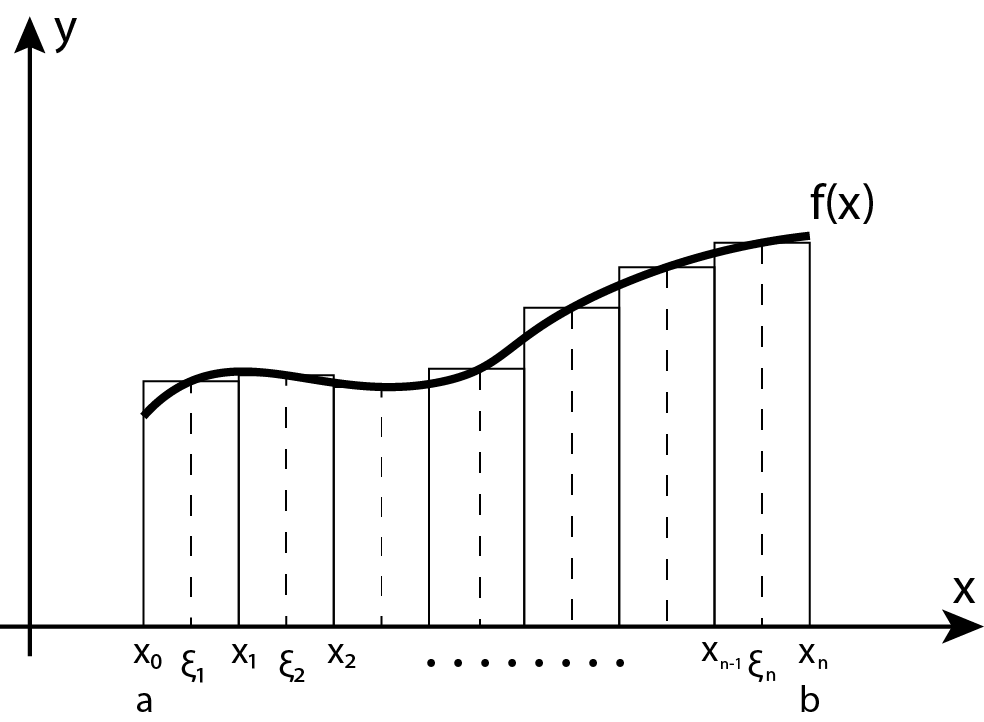
\includegraphics[scale=0.7]{graph1.png}\label{figure1}
        \end{center}
    \end{figure}

    $\Delta i = [x_{i-1}, x_{i}], \quad \Delta x = x_{i} - x_{i-1}$ - длина отрезка $\Delta i$.\\

    Составим сумму $S_{n} = \sum_{i=1}^{n} f(\xi_{i})\Delta x_{i}$, где $f(\xi_{i})$ - высота $i$-го прямоугольника и
    $\Delta x_{i}$ - ширина $i$-го прямоугольника.\\

    $S_{n}$ - площадь ступенчатой фигуры, составленной из прямоугольников под графиком функции $f(x)$.\\

    Говорят, что функция $f$ интегрируема на $[a;b]$, если существует предел интегральных сумм $S_{n}$, то есть
    $\exists \underset{max\Delta x_{i}\rightarrow0}{\lim}S_{n}$, причем этот предел не зависит ни от способа разбиения
    отрезка $[a;b]$, ни от способа выбора точек $\xi_{i}$.\\

    Этот предел называется \textbf{интегралом Римана} функции $f$ на $[a;b]$. Класс интегрируемых функций на отрезке
    $[a;b]$ будем обозначать $R([a;b])$.
\end{definition}

\section{База на множестве}

\begin{definition}[база множества]
    Пусть $X$ - произвольное множество.\\

    Система $\beta$ подмножеств множества $X$ называется \textbf{базой} на $X$, если:
    \begin{enumerate}
        \item $\forall \beta \in \beta \quad \beta \ne \o$
        \item $\forall \beta_{1}, \beta_{2} \in \beta \ \exists \beta_{3} \in \beta: \quad \beta_{3} \subset \beta_{1}
                  \cap \beta_{2}$
    \end{enumerate}
\end{definition}

\begin{example}[баз множества]
    \begin{enumerate}
        \item $\beta = \{X\}$ - база
        \item $X = \mathbb{R}, \quad \beta = \{\beta_{n} = (-\frac{1}{n};\frac{1}{n}), \ n \in \mathbb{N}\}$
        \item $X = \mathbb{R}, \quad \beta = \{\beta_{\epsilon} = \{x: \  0 < |x| < \epsilon\}, \epsilon > 0\}$
              (выколотые окрестности нуля)
    \end{enumerate}
\end{example}

\section{Предел функции по базе (в том числе, для метрических пространств)}

\begin{definition}[предел по базе]
    Пусть $f:X\rightarrow\mathbb{R}, \ \beta$ - база на $X$\\

    Число $A\in\mathbb{R}$ называется \textbf{пределом} функции $f$ \textbf{по базе $\beta$}, если
    $\forall \epsilon > 0 \ \exists$ элемент базы $\beta \in \beta: \quad |f(x) - A| < \epsilon$.
    \begin{equation*}
        \underset{\beta}{\lim} f(x)
    \end{equation*}
\end{definition}

\begin{definition}[предел по базе (МП)]
    Пусть $(Y, d)$ - МП, $f:X\rightarrow Y, \ \beta$ - база на $X$.\\

    $y\in Y$ называется \textbf{пределом} функции $f(x)$ \textbf{по базе $\beta$}, если $\forall \epsilon > 0 \
        \exists \beta \in \beta \ \forall x \in \beta: \quad d(f(x), y) < \epsilon$, или, что то же самое,
    $\forall V_{Y}(y) \ \exists \beta \in \beta \quad f(\beta) \subset V_{Y}(y)$, где $V_{Y}$ - окрестность
    метрического пространства $Y$.
\end{definition}

\section{Основные свойства предела по базе}

\begin{theorem}[основные свойства предела по базе]
    Пусть $f:X\rightarrow\mathbb{R}, \ \beta$ - база на $X$:
    \begin{enumerate}
        \item Если $\exists \underset{\beta}{\lim}f(x)$, то $\exists \beta \in \beta: \ f$ ограничена на $\beta$
        \item Если $\underset{\beta}{\lim}f(x) = A$ и $\underset{\beta}{\lim}f(x) = B$, то $A = B$
    \end{enumerate}
\end{theorem}

\section{Связь предела функции по базе с неравенствами}

\begin{theorem}[связь предела функции по базе с неравенствами]
    Пусть $f:X\rightarrow\mathbb{R}, \ g:X\rightarrow\mathbb{R}, \ \beta$ - база на $X$:
    \begin{enumerate}
        \item Если $\exists\beta\in\beta: \quad \forall x \in \beta \ f(x) \leqslant g(x)$, то $\underset{\beta}
                  {\lim}f(x) \leqslant \underset{\beta}{\lim}g(x)$
        \item Если $\underset{\beta}{\lim}f(x) < \underset{\beta}{\lim}g(x)$, то $\exists\beta\in\beta \ \forall
                  x \in \beta \quad f(x) < g(x)$\\

              Если $\underset{\beta}{\lim}f(x) \geqslant \underset{\beta}{\lim}g(x)$, то $\exists\beta\in\beta \ \forall
                  x \in \beta \quad f(x) \geqslant g(x)$
        \item Если $h:X\rightarrow \mathbb{R}$ и $\exists\beta\in\beta: \ \forall x \in \beta \ f(x) \leqslant h(x)
                  \leqslant g(x)$ \textbf{И} $A = \underset{\beta}{\lim}f(x) = \underset{\beta}{\lim}g(x)$, то $\underset{\beta}
                  {\lim}h(x) = A$
    \end{enumerate}
\end{theorem}

\section{Критерий Коши существования предела по базе}

\begin{theorem}[критерий Коши существования предела по базе]
    Существуют две формулировки:
    \begin{enumerate}
        \item Пусть $f:X\rightarrow\mathbb{R}, \ \beta$ - база на $X$.

              Функция $f(x)$ имеет предел по базе $\beta \iff \forall \epsilon > 0 \ \exists\beta\in\beta: \quad \forall
                  x_{1},x_{2} \in \beta \ |f(x_{1}) - f(x_{2})| < \epsilon$

        \item Пусть $(Y,d)$ - МП (\textbf{полное}), $f:X\rightarrow Y, \ \beta$ - база на $Y$.

              Функция $f(x)$ имеет предел по базе $\beta \iff \forall \epsilon>0\exists\beta\in\beta: \quad \forall
                  x_{1},x_{2} \in \beta \ d(f(x_{1}), f(x_{2})) < \epsilon$
    \end{enumerate}
\end{theorem}

\section{Разбиение с отмеченными точками}

\begin{definition}[разбиение]
    Пусть дан отрезок $[a;b]$. \textbf{Разбиением} $P$ отрезка $[a;b]$ называется набор точек $a=x_{0}<x_{1}<\ldots
        <x_{n-1}<x_{n}=b$. То есть $P = \{x_{0},\ldots,x_{n}\}$. Отрезки $[x_{i-1};x_{i}] = \Delta_{i}$.
    $x_{i}-x_{i-1} = \Delta x_{i}$ - длина $i$-го отрезка разбиения $\lambda(P) = \underset{i=\overline{0,n}}
        {\max}\{\Delta x_{i}\}$. Величины $\Delta_{i}, \Delta x_{i}, \lambda(P)$ - параметры ограничения.
\end{definition}

\begin{definition}[разбиение с отмеченными точками]
    \textbf{Разбиением с отмеченными точками} называется пара наборов
    \begin{equation*}
        P(\xi) = \{x_{0},\ldots,x_{n}\},\{\xi_{0},\ldots,\xi_{n}\},
    \end{equation*}
    \center{где $a=x_{0} < \ldots < x_{n}=b, \ \xi_{i}\in [x_{i-1};x_{i}]$.}
    \begin{figure}[h]
        \begin{minipage}[h]{0.49\linewidth}
            \center{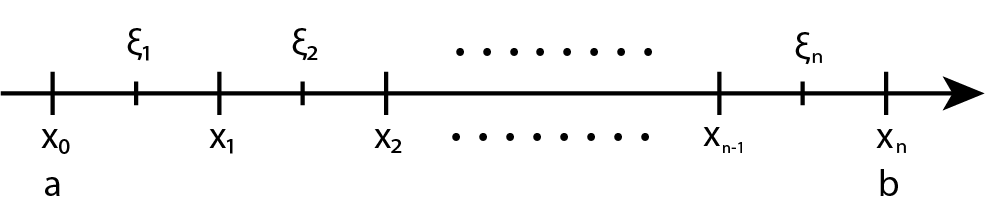
\includegraphics[scale=0.6]{graph2.png}}
        \end{minipage}
        \hfill
        \begin{minipage}[h]{0.49\linewidth}
            Пусть $\Re_{\xi} = \{(P,\xi)\}$ - семейство всевозможных разбиений с отмеченными точками отрезка $[a,b]$.
        \end{minipage}
    \end{figure}
\end{definition}

\section{База на множестве разбиений отмеченными точками}

\begin{statement}
    Множество $\beta = \{\beta_{\delta}:\quad \delta > 0\}$ является базой на $\Re_{\xi}$.
\end{statement}

\section{Интегрируемая по Риману функция, интеграл Римана (через предел по базе)}

\begin{definition}[!]
    Пусть $f:[a;b]\rightarrow\mathbb{R}, \ (P,\xi)$ - разбиение отрезка $[a;b]$ с отмеченными точками. Составим сумму:
    \begin{equation*}
        \sigma(f,(P,\xi)) = \sum_{k=1}^{n}f(\xi_{k})\Delta x_{k}
    \end{equation*}
    Можно смотреть на $\sigma$ для фиксированной функции $f(x)$ как на функцию, сопоставляющую разбиение $(P,\xi)\in
        \Re_{\xi}$ сумме $\sum_{k=1}^{n}f(\xi_{k})\Delta x_{k}$, то есть $\sigma_{f}:\Re_{\xi}\rightarrow\mathbb{R}$
    (то есть $(P,\xi)$ - аргумент функции $\sigma$).\\

    Говорят, что функция $f:[a;b]\rightarrow\mathbb{R}$ интегрируема по Риману на $[a;b]$, если:
    \begin{equation*}
        \exists\underset{\lambda(P)\rightarrow0}{\lim}\sigma_{f}((P,\xi)) = \underset{\lambda(P)\rightarrow0}{\lim}
        \sum_{k=1}^{n}f(\xi_{k})\Delta x_{k}
    \end{equation*}
    Или, что то же самое, если $\forall\epsilon>0 \ \exists\delta>0$ и соответствующий элемент $\beta_{\delta} \in
        \beta:\quad \forall$ разбиения $(P,\xi): \ \lambda(P) < \delta$ выполняется неравенство \\ $| \sigma_{f}
        ((P,\xi)) - I | < 0$:
    \begin{equation*}
        I = \underset{\lambda(P)\rightarrow0}{\lim}\sigma_{f}((P,\xi)) = \int_{a}^{b}f(x)dx
    \end{equation*}
\end{definition}

\section{Необходимое условие интегрируемости функции}

\begin{theorem}[необходимое условие интегрируемости функции]
    $*\_*$

    Если $f:[a;b]\rightarrow\mathbb{R}$ интегрируема на $[a;b]$ (то есть $f\in\mathbb{R}[a;b]$), то \\ $f$
    ограничена на $[a;b]$.
\end{theorem}

\section{Суммы Дарбу}

\begin{definition}[нижняя/верхняя суммы Дарбу]
    Пусть $f[a;b] \rightarrow \mathbb{R}, \ P$ - произвольное разбиение отрезка $[a;b]$. Числа
    $\underline{S}(P) = \sum_{k=1}^{n}m_{k}\Delta x_{k}$ и $\overline{S}(P) = \sum_{k=1}^{n}M_{k}
        \Delta x_{k}$, где $m_{k} = \underset{\xi \in \Delta k}{\inf}f(\xi), \ M_{k} = \underset{\xi\in\Delta k}
        {\sup}f(\xi)$, называются \textbf{нижней} и \textbf{верхней суммами Дарбу}, отвечающими разбиению $P$.

    \begin{figure}[h]
        \begin{minipage}[h]{0.49\linewidth}
            \center{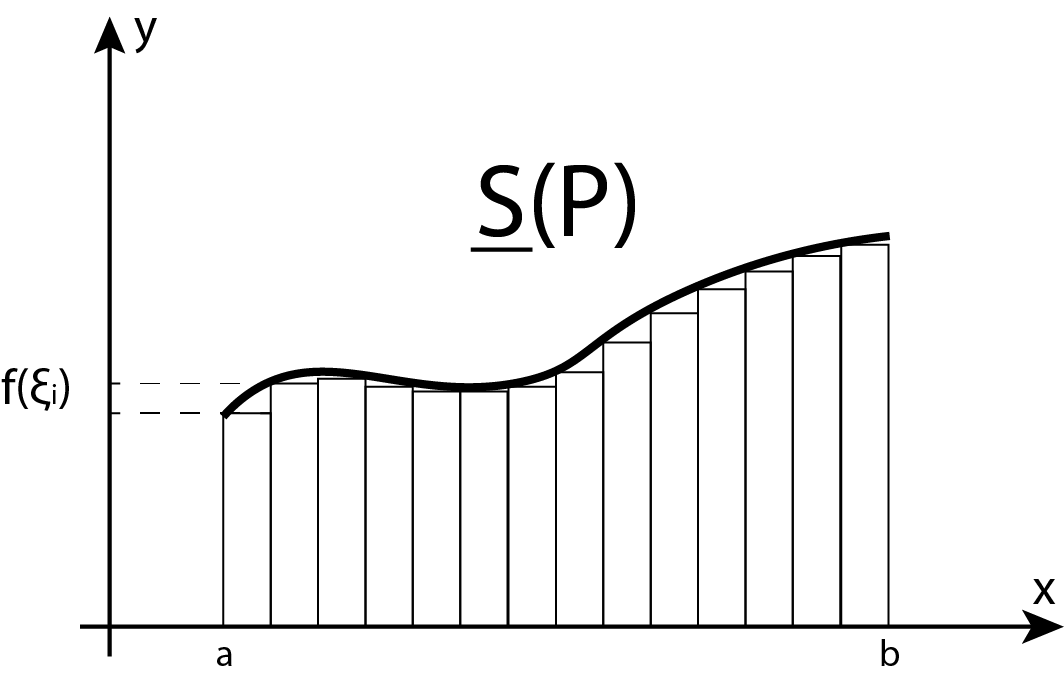
\includegraphics[scale=0.6]{graph4.png}}
        \end{minipage}
        \hfill
        \begin{minipage}[h]{0.49\linewidth}
            \center{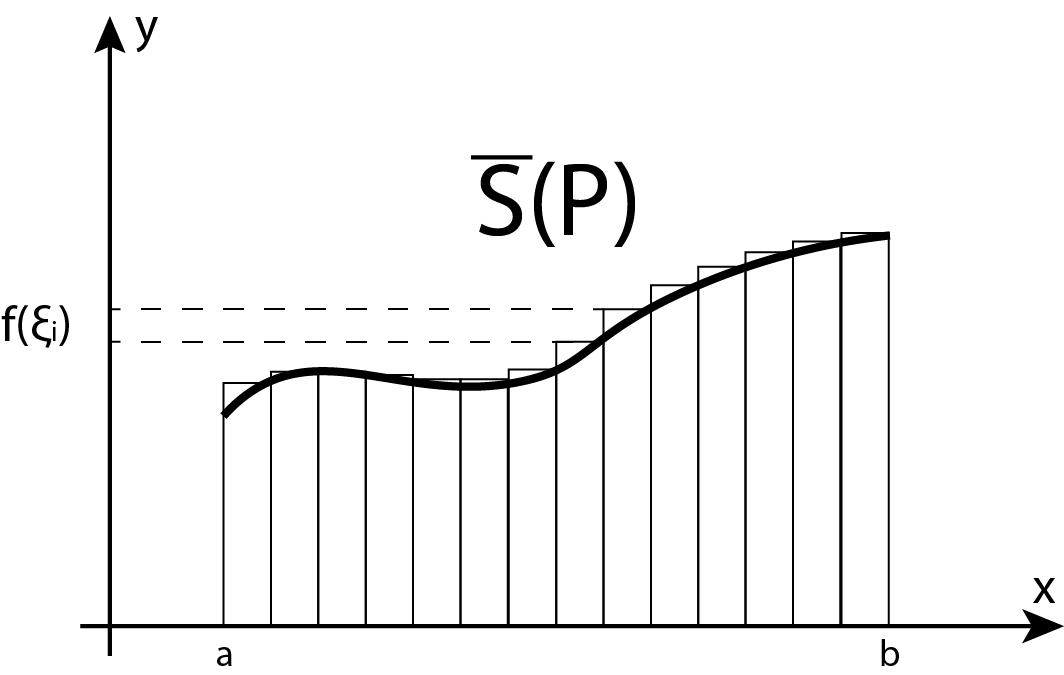
\includegraphics[scale=0.6]{graph3.png}}
        \end{minipage}
    \end{figure}
\end{definition}

\section{Свойства сумм Дарбу}

\begin{theorem}[свойства сумм Дарбу]
    Свойства:
    \begin{enumerate}
        \item $\forall(P,\xi) \ \underline{S}(P)\leqslant\sigma_{f}((P,\xi))\leqslant\overline{S}(P)$
        \item Если разбиение $P'$ получено из разбиения $P$ добавлением новых точек, то $\underline{S}
                  (P') \geqslant \underline{S}(P)$ и $\overline{S}(P')\leqslant\overline{S}(P)$
        \item $\forall P_{1},P_{2} \quad \underline{S}(P_{1})\leqslant\overline{S}(P_{2})$
    \end{enumerate}
\end{theorem}

\section{Нижний и верхний интегралы Дарбу}

\begin{definition}[верхний/нижний интеграл Дарбу]
    Числа $\underline{\mathfrak{I}}=\sup\underline{S}(P)$ и $\overline{\mathfrak{I}}=\inf\overline{S}(P)$ называются
    \textbf{нижним} и \textbf{верхним интегралом Дарбу}.
\end{definition}

\section{Критерий интегрируемости}

\begin{theorem}[критерий интегрируемости]
    Функция $f:[a;b]\rightarrow\mathbb{R}$ интегрируема на $[a;b] \iff \underset{\lambda (P)\rightarrow0}{\lim}
        (\overline{S}(P) - \underline{S}(P)) = 0$.
\end{theorem}

\section{Колебание функции на отрезке}

\begin{definition}
    Обозначим $M_{i} - m_{i} = \underset{\xi \in \Delta i}{\sup}f(\xi) - \underset{\xi\in\Delta i}{\inf}f(\xi)
        = \underset{x_{1},x_{2}\in\Delta i}{\sup}| f(x_{1}) - f(x_{2}) | = \omega_{i} = \omega_{i}(f,\Delta i)$.

    $\omega_{i}$ называется \textbf{колебанием} функции $f(x)$ на отрезке $\Delta i$.

    $\overline{S}(P) - \underline{S}(P) = \sum_{i = 1}^{n}\omega_{i}\Delta x_{i}$
\end{definition}

\section{Теорема Дарбу}

\begin{theorem}[Дарбу]
    Для любой ограниченной функции $f:[a;b]\rightarrow\mathbb{R}$ выполняются равенства:

    \begin{center}
        {\large $\underline{\mathfrak{I}} = \underset{\lambda(P)\rightarrow0}{\lim}\underline{S}(P); \ \overline{\mathfrak{I}}
                = \underset{\lambda(P)\rightarrow0}{\lim}\overline{S}(P)$}
    \end{center}
\end{theorem}

\section{Интегрируемость непрерывных функций}

\begin{theorem}[интегрируемость непрерывных функций]
    Пусть $f:[a;b]\rightarrow\mathbb{R}$ непрерывна на $[a;b]\implies f$ - интегрируема на $[a;b]$
    , то есть $f\in\mathbb{R}[a;b]$.
\end{theorem}

\section{Интегрируемость функции с конечным числом точек разрыва}

\begin{theorem}[интегрируемость функций с конечным числом точек разрыва]
    Пусть $f:[a;b]\rightarrow\mathbb{R}$ - ограничена и имеет на $[a;b]$ конечное число точек
    разрыва. Тогда $f\in\mathbb{R}[a;b]$ интегрируема на $[a;b]$.
\end{theorem}

\section{Интегрируемость монотонных функций}

\begin{theorem}[интегрируемость монотонных функций]
    Пусть $f:[a;b]\rightarrow\mathbb{R}$ - монотонна на $[a;b]\implies f$ - интегрируема на $[a;b]$.
\end{theorem}

\section{Свойства интегрируемых функций}

\begin{theorem}
    Пусть $f\in\mathbb{R}[a;b], \ g\in\mathbb{R}[a;b]$. Тогда:
    \begin{enumerate}
        \item $f\pm g \in R[a;b]$.
        \item $\alpha f \in R[a;b], \ \alpha \in \mathbb{R}$.
        \item $f*g\in R[a;b]$.
        \item $|f|\in R[a;b]$, при этом:
              \begin{itemize}
                  \item $\int_{a}^{b}(f\pm g)dx = \int_{a}^{b}f(x)dx \pm \int_{a}^{b}g(x)dx$
                  \item $\int_{a}^{b}\alpha f(x)dx = \alpha \int_{a}^{b}f(x)dx$
                  \item $|\int_{a}^{b}f(x)dx | \leqslant \int_{a}^{b}|f(x)|dx$
              \end{itemize}
    \end{enumerate}
\end{theorem}

\section{Аддитивность интеграла Римана}

\begin{definition}
    Пусть $a>b, \ a,b\in\mathbb{R}$, положим $\int_{a}^{b}f(x)dx = -\int_{b}^{a}f(x)dx$. Если $a=b$, то
    $\int_{a}^{a=b}f(x)dx =0$.
\end{definition}

\begin{theorem}[Аддитивность интеграла Римана]
    Пусть даны точки $a,b,c\in \mathbb{R}$. Если $f$ - интегрируема на большем из отрезков $[a;b],\ [a,c],\
        [b,c]$, то $f$ - интегрируема и на меньших отрезках. И наоборот, если $f$ интегрирема на двух меньших отрезках,
    то она интегрируема и на большем отрезке. При этом:
    \begin{equation*}
        \int_{a}^{b}f(x) dx + \int_{b}^{c}f(x)dx + \int_{c}^{a}f(x)dx = 0
    \end{equation*}
\end{theorem}

\section{Монотонность интеграла Римана и ее следствия}

\begin{theorem}
    Если $a<b$ и $f\in R[a;b]$ и:
    \begin{enumerate}
        \item $\forall x \in [a;b] \ f(x) \geqslant 0$, то $\int_{a}^{b} f(x) dx \geqslant 0$
        \item $\forall x \in [a;b] \ f(x) > 0$, то $\int_{a}^{b}f(x)dx > 0$
    \end{enumerate}
\end{theorem}

\begin{effect}
    (теоремы 2.4.9)
    \begin{enumerate}
        \item Если $a<b, \ f,g \in R[a;b]$ и:
              \begin{enumerate}
                  \item $\forall x \in [a;b] \ f(x) \leqslant g(x)$, то $\int_{a}^{b}f(x) dx \leqslant
                            \int_{a}^{b}g(x)dx$
                  \item $\forall x \in [a;b] \ f(x) < g(x)$, то $\int_{a}^{b}f(x)dx < \int_{a}^{b}g(x) dx$
              \end{enumerate}
        \item Если $f\in R[a;b], \ a<b, \ M = \underset{x \in [a;b]}{\sup}f(x), \ m = \underset{x\in[a;b]}
                  {\inf}f(x)$, то $m(b-a) \leqslant \int_{a}^{b}f(x)dx \leqslant M(b-a)$.
        \item (Теорема о среднем)

              Пусть $f\in R[a;b] (a>b, a<b), \ m = \underset{x \in[a;b]}{\inf}f(x), \ M = \underset{x \in[a;b]}{\sup}f(x)$.
              Тогда существует $\mu \in [m;M]: \ \int_{a}^{b}f(x)dx = \mu (b-a)$.

              \begin{effect}
                  Если, кроме того, $f(x)$ - непрерывна на $[a;b]$, то $\exists c \in [a;b]: \ \int_{a}^{b}f(x)dx =
                      f(x)(b-a)$.
              \end{effect}

    \end{enumerate}
\end{effect}

\section{Теорема о среднем}

Пусть $f\in R[a;b] (a>b, a<b), \ m = \underset{x \in[a;b]}{\inf}f(x), \ M = \underset{x \in[a;b]}{\sup}f(x)$.
Тогда существует $\mu \in [m;M]: \ \int_{a}^{b}f(x)dx = \mu (b-a)$.

\begin{effect}
    Если, кроме того, $f(x)$ - непрерывна на $[a;b]$, то $\exists c \in [a;b]: \ \int_{a}^{b}f(x)dx =
        f(x)(b-a)$.
\end{effect}

\section{Первая теорема о среднем}

\begin{theorem}[Первая теорема о среднем]
    Пусть $f,g\in R[a;b] (a>b, a<b), \ m = \underset{x\in[a;b]}{\inf}f(x), \ M = \underset{x\in[a;b]}{\sup}f(x)$
    и $g$ не меняет свой знак на $[a;b]$. Тогда $\exists \mu \in [m;M]: \ \int_{a}^{b}f(x)g(x)dx = \mu \int_{a}^{b}
        g(x)dx$.
\end{theorem}

\section{Интеграл Римана как функция верхнего предела интегрирования}

\begin{definition}
    Пусть $f\in R[a;b], \ x \in [a;b]$.

    Рассмотрим функцию $F(x) = \int_{a}^{x}f(t)dt, \ F(x)$ определена для $\forall x \in [a;b]$.
\end{definition}

\section{Непрерывность интеграла Римана}

\begin{theorem}[непрерывность интеграла Римана]
    Если $f\in R[a;b]$, то $F(x) = \int_{a}^{x}f(t)dt$ - непрерывна на $[a;b]$.
\end{theorem}

\section{Дифференцируемость интеграла Римана по верхнему пределу и ее следствие}

\begin{theorem}[о дифференцируемости интеграла Римана как функции по верхнему пределу]
    Пусть $f\in R[a;b], \ x \in [a;b]$ и $f$ непрерывна в точке $x$, тогда функция $F(x) = \int_{a}^{x}f(t)dt$
    дифференцируема в точке $x$, причем:
    \begin{equation*}
        F'(x) = f(x) \implies (\int_{a}^{x}f(t)dt)_{x}'=f(x)
    \end{equation*}
\end{theorem}

\begin{effect}
    Если $f$ - непрерывна на $[a;b]$, то на $[a;b]$ она имеет первообразную, которая равна:
    \begin{equation*}
        \Phi (x) = \int_{a}^{x}f(t)dt + C
    \end{equation*}
\end{effect}

\begin{remark}
    Рассмотрим следующие классы (множества/пространства) функций:
    \begin{itemize}
        \item $R[a;b]$ - множество интегрируемых на $[a;b]$ функций;
        \item $C[a;b]$ - множество непрерывных на $[a;b]$ функций;
        \item $C^{o}[a;b]$ - множество дифференцируемых на $[a;b]$ функций.
    \end{itemize}
    Получаем:
    \begin{equation*}
        C^{o}[a;b]\subset C[a;b] \subset R[a;b].
    \end{equation*}
\end{remark}

\section{Вторая теорема о среднем}

\begin{theorem}[вторая теорема о среднем]
    Пусть $f,g\in R[a;b]$, причем $f$ - монотонна на $[a;b]$. Тогда $\exists \xi \in [a;b]:$
    \begin{equation*}
        \int_{a}^{b}f(x)g(x)dx = f(a)\int_{a}^{\xi}g(x)dx + f(b)\int_{\xi}^{b}g(x)dx
    \end{equation*}
\end{theorem}

\section{Формула Ньютона-Лейбница для непрерывной функции}

\begin{theorem}
    Пусть $f$ - непрерывна на $[a;b]$ и $F(x)$ - её первообразная.

    Тогда $\int_{a}^{b}f(x)dx = F(b) - F(a) = F(x)|_{a}^{b}$
\end{theorem}

\section{Формула Ньютона-Лейбница для функции, недиффиренцируемой в
  некоторых (конечное число) точках отрезка. Следствие.}

\begin{theorem}
    Пусть $F(x)$ - непрерывна на $[a;b]$, дифференцируема на $[a;b]$
    за исключением не более чем конечного числа точек. Причем всюду, где
    она дифференцируема: $F'(x) = f(x)$. И, наконец, $f(x)\in R[a;b]$.

    Тогда:
    \begin{equation*}
        \int_{a}^{b}f(x)dx = F(b) - F(a) = F(x)|_{a}^{b}
    \end{equation*}
\end{theorem}

\begin{effect}
    Если функция $F(x)$ удовлетворяет условиям теоремы 2.5.2, то $\forall x \in [a;b]:$
    \begin{equation*}
        F(x) = F(a) + \int_{a}^{x}F'(t)dt.
    \end{equation*}
\end{effect}

\section{Формула интегрирования по частям для определенного интеграла}

\begin{theorem}[формула интегрирования по частям]
    Если фукнции $u(x)$ и $v(x)$ непрерывно дифференцируемы на отрезке $[a;b]$, то
    справедливо равенство:
    \begin{equation*}
        \int_{a}^{b}udv = uv|_{a}^{b} - \int_{a}^{b}vdu.
    \end{equation*}
\end{theorem}

\section{Формула Тейлора с остаточным членом в интегральной форме}

\begin{theorem}[формула Тейлора с остаточным членом в интегральной форме]
    Пусть функция $f(t)$ имеет на отрезке $[a;x]$ непрерывные производные до
    $n$-го порядка включительно. Тогда справедлива формула Тейлора:
    \begin{equation*}
        f(x) = f(a) + \frac{f'(a)}{1!}(x-a) + \frac{f''(a)}{2!}(x-a)^{2} + \ldots +
        \frac{f^{(n-1)}(a)}{(n-1)!}(x-a)^{n-1} + r_{n}(a;x),
    \end{equation*}
    где $r_{n}(a;x) = \frac{1}{(n-1)!}\int_{a}^{x}f^{(n)}(t)(x-a)^{n-1}dt$.
\end{theorem}

\section{Замена переменной в интеграле Римана (для непрерывных функций)}

\begin{theorem}
    Пусть $\phi : [\alpha;\beta] \rightarrow [a;b]$ - непрерывно дифференцируемое
    отображение отрезка $[\alpha;\beta]$ в отрезок $[a;b]$, причем $\phi(\alpha)
        = a, \ \phi(\beta) = b$. Тогда для любой функции $f(x)$, непрерывной на $[a;b]$,
    функция $f(\phi(t))\phi'(t)$ - непрерывна на $[\alpha;\beta]$ и справедливо
    равенство:
    \begin{equation*}
        \int_{a}^{b}f(x)dx = \int_{\alpha}^{\beta}f(\phi(t))\phi'(t)dt.
    \end{equation*}
\end{theorem}

\section{Замена переменной в интеграле Римана (для интегрируемых функций)}

\begin{theorem}[замена переменной для интегрируемых функций]
    Пусть $f:[a;b]\rightarrow\mathbb{R}, \ f\in R[a;b]$, функция $x = \phi(t):$
    \begin{enumerate}
        \item $\phi:[\alpha;\beta]\rightarrow[a;b]$
        \item $\phi(\alpha)=a, \ \phi(\beta)=b$
        \item $\phi'(t)$ непрерывна на $[\alpha;\beta]$
        \item $\phi$ - строго монотонна
    \end{enumerate}
    Тогда:
    \begin{equation*}
        \int_{a}^{b}f(x)dx = \int_{\alpha}^{\beta}f(\phi(t))\phi'(t)dt
    \end{equation*}
\end{theorem}

\section{Путь}

\begin{definition}
    Пусть $(X,\rho)$ - метрическое пространство, $[a;b] \subset \mathbb{R}$. Будем называть \textbf{путем}
    произвольное непрерывное отображение:
    \begin{equation*}
        \gamma:[a;b]\rightarrow X
    \end{equation*}
\end{definition}

\section{Простой путь}

\begin{definition}
    Пусть $\gamma:[a;b]\rightarrow X$ называется \textbf{простым}, если:
    \begin{equation*}
        \forall t_1,t_2 \in[a;b]: \quad \gamma(t_1) = \gamma(t_2) \implies t_1 = t_2
    \end{equation*}
    \begin{figure}[H]
        \begin{center}
            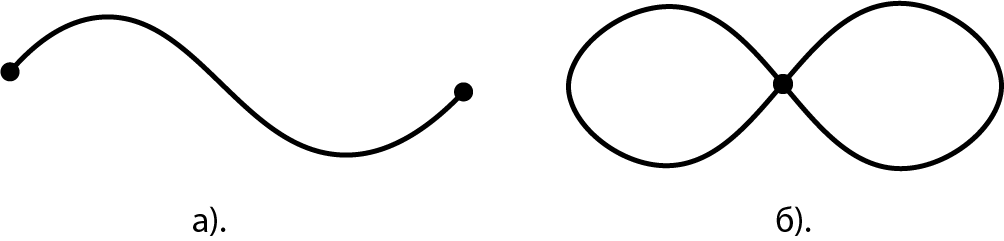
\includegraphics[scale=0.2]{graph6.png}\label{figure6}

            а). простой путь $\quad$ б). непростой путь
        \end{center}
    \end{figure}
\end{definition}

\section{Отношение эквивалентности путей}

На множестве путей введем отношение.

Пусть $\gamma_1:[a;b]\rightarrow X, \ \gamma_2:[\alpha;\beta] \rightarrow X$.

Будем говорить, что $\gamma_1$ и $\gamma_2$ находятся в отношении $"\sim"$, то есть $\gamma_1 \sim \gamma_2$,
если существует строго возрастающее отображение $\phi:[\alpha;\beta]\rightarrow[a;b]:$
\begin{equation*}
    \phi(\alpha) = a, \ \phi(\beta) = b,
\end{equation*}
а так же:
\begin{equation*}
    \gamma_2(\tau) = \gamma_1(\phi(\tau))
\end{equation*}
\begin{figure}[H]
    \begin{center}
        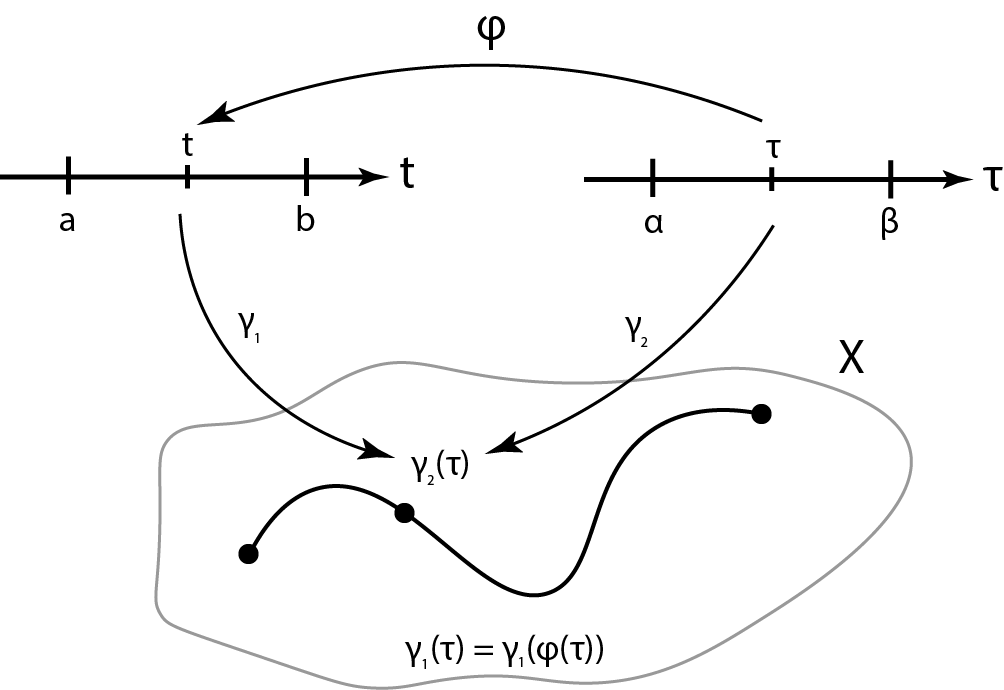
\includegraphics[scale=0.2]{graph7.png}\label{figure7}
    \end{center}
\end{figure}

\section{Носитель пути}

\begin{definition}
    Образ пути $\gamma$ называется \textbf{носителем} этого пути.
\end{definition}

\begin{example}
    Рассмотрим:

    $\gamma_1: [0;1] \rightarrow \mathbb{R}: \quad \gamma_1(t) = t$;

    $\gamma_2: [0;1] \rightarrow \mathbb{R}: \quad \gamma_2(\tau) = \tau^3$,

    \begin{figure}[H]
        \begin{center}
            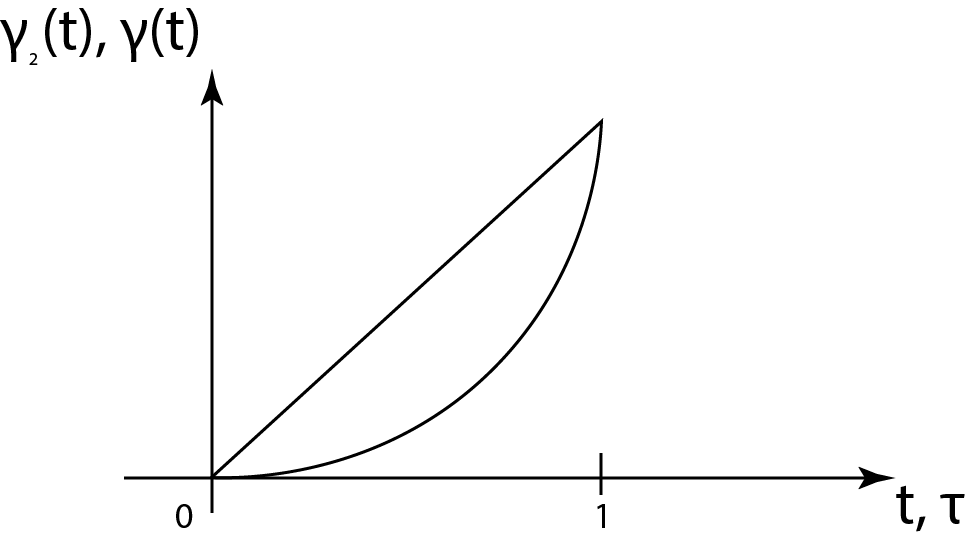
\includegraphics[scale=0.2]{graph8.png}\label{figure8}
        \end{center}
    \end{figure}

    Что бы доказать, что $\gamma_1 \sim \gamma_2$, нужно найти строго возрастающее отображение
    $\phi:[0;1]\rightarrow[0;1]$:

    $t = \phi(\tau) = \tau^3, \ \phi(\tau)$ - строго возрастающее, $\phi(0) = 0, \ \phi(1) = 1$;

    $\gamma_2(\tau) = \tau^3 = \phi(\tau) = t = \gamma_1(t) = \gamma_1(\phi(\tau)) \implies
        \gamma_2(\tau) = \gamma_1(\phi(\tau))$.
\end{example}

\section{Кривая на множестве}

\begin{definition}
    \textbf{Кривой} в $X$ будем называть класс эквивалентных путей.
\end{definition}

\section{Простая кривая}

\begin{definition}
    Кривая называется \textbf{простой}, если она представляется простым путем (это значит, что в ее классе
    есть простой путь).
\end{definition}

\section{Параметризация кривой}

\begin{definition}
    Путь, представляющий данную кривую (из класса эквивалентности путей) $l$ называется
    \textbf{параметризацией} этой кривой.
\end{definition}

\section{Гладкая параметризация кривой}

\begin{definition}
    Пусть $l$ - простая кривая в $\mathbb{R}^2, \ \gamma(t) = (x(t);t(t))$ - ее параметризация.
    Кривая $l$ называется \textbf{гладкой}, если $\forall t \ x(t),y(t)$ имеют непрерывные производные
    на $[\alpha,\beta]$ и $\nexists t_0 \in [\alpha,\beta] \ (\gamma : [\alpha,\beta] \rightarrow
        \mathbb{R}^2), \ x'(t_0)=0$ и $y'(t_0) = 0$.
\end{definition}

\section{Ломаная, вписанная в кривую}

\begin{definition}
    Пусть $l \subset \mathbb{R}^2 \ (\mathbb{R}^3)$ и $\gamma:[\alpha,\beta]\rightarrow\mathbb{R}^2 \
        (\mathbb{R}^3)$ - параметризация кривой $l$.

    Пусть $\alpha = t_0 < t_1 < \ldots < t_{n-1} < t_n = \beta$ - разбиение отрезка $[\alpha,\beta]$
    и $M_i = \gamma(t_i), \ i=\overline{0,n}$ - точка пути $\gamma$ (кривая $l$):
    \begin{equation*}
        M_i = \gamma (t_i) = (x(t_i);y(t_i))
    \end{equation*}
    Тогда отрезок $M_{i-1}M_i \ (i = \overline{1,n})$ называется \textbf{звеном} кривой $l$.
    Объединение $\underset{i}{\cap}M_{i-1}M_i$ - \textbf{ломаная, вписанная в $l$}.
\end{definition}

\section{Периметр ломаной, вписанной в кривую}

\begin{definition}
    \textbf{Периметром} ломаной называется сумма длин ее звеньев:
    \begin{equation*}
        p(M_0,M_1,\ldots,M_n) = \sum_{i=1}^{n}| M_{i-1}M_i |
    \end{equation*}
    \begin{figure}[h]
        \begin{minipage}[h]{0.49\linewidth}
            \center{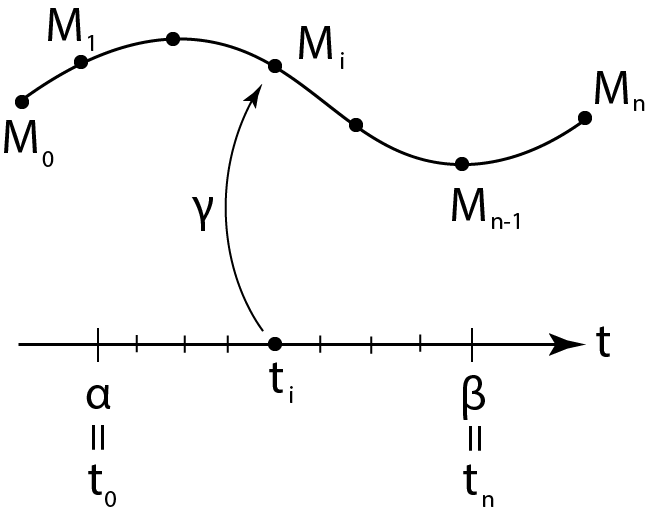
\includegraphics[scale=0.2]{graph9.png}}
        \end{minipage}
        \hfill
        \begin{minipage}[h]{0.49\linewidth}
            \center{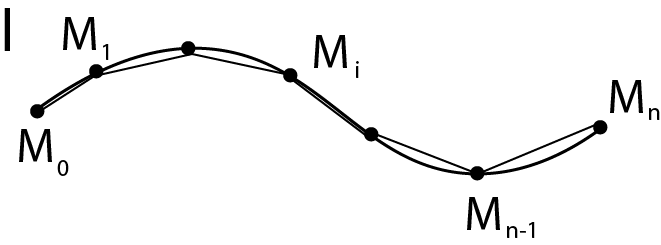
\includegraphics[scale=0.2]{graph10.png}}
        \end{minipage}
    \end{figure}
\end{definition}

\clearpage

\section{Спрямляемая кривая}

\begin{definition}
    Если множество периметров ломаных, вписанных в данную кривую $l$ - ограничено, то кривую $l$
    будем называть \textbf{спрямляемой}.
\end{definition}

\section{Аддитивность длины кривой}

\begin{theorem}[аддитивность длины кривой]
    Функция $S(l)$ является аддитивной, то есть если $l = l_1 \cup l_2$, то $S(l) = S(l_1) + S(l_2)$.

    \textbf{Более тонко:} Пусть $\gamma:[a;b]\rightarrow\mathbb{R}^2$ - параметризация спрямляемой кривой
    $l$, точка $c \in [a;b]$:

    $\gamma_1:[a;c] \rightarrow \mathbb{R}^2$ - параметризация кривой $l_1$,

    $\gamma_2:[c;b] \rightarrow \mathbb{R}^2$ - параметризация кривой $l_2$,

    при этом $C = \gamma(c) = \gamma_1(c) = \gamma_2(c)$.
    \begin{figure}[H]
        \begin{center}
            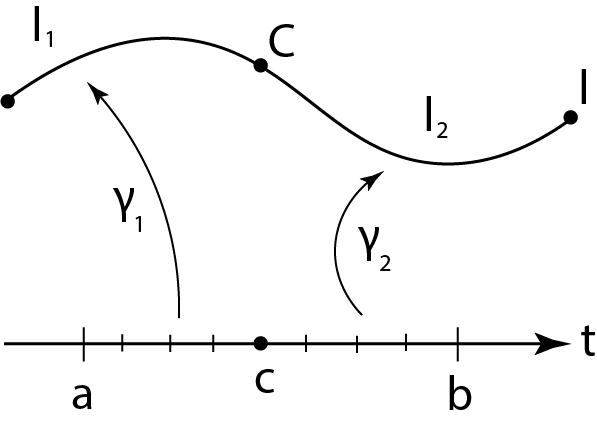
\includegraphics[scale=0.2]{graph12.png}\label{figure12}
        \end{center}
    \end{figure}

    Тогда $S(l) = S(l_1) + S(l_2)$.
\end{theorem}

\section{Длина кривой как предел}

\begin{theorem}
    Пусть $l$ - простая спрямляемая незамкнутая кривая в $\mathbb{R}^2$ и $\gamma:[a;b]\rightarrow\mathbb{R}^2$
    - ее параметризация. Пусть $a = t_0 < t_1 < \ldots < t_{n-1} < t_n = b$ - разбиение отрезка $[a;b]$,
    этому разбиению соответствуют точки $M_0,M_1,\ldots,M_n$ - соответсвующая ломаная, вписанная в $l \
        (M_i = \gamma(t_i))$, тогда:
    \begin{equation*}
        S(l) = \underset{\lambda\rightarrow0}{\lim}p(m),
    \end{equation*}
    где $\lambda = \underset{i}{\max}\Delta t_i, \ \Delta t_i = t_i - t_{i-1}$.
\end{theorem}

\section{Формула вычисления длины кривой}

\begin{theorem}[формула для вычисления длины кривой]
    Пусть $l$ - гладкая кривая; $\gamma:[a;b]\rightarrow\mathbb{R}^2$ - ее параметризация (гладкая,
    то есть $\gamma(t) = (x(t);y(t))$, где $x(t)$ и $y(t)$ имеют непрерывные произведения на $[a;b]$).
    Тогда $l$ - спрямляема и:
    \begin{equation*}
        S(l) = \int_{a}^{b}\sqrt{(x'(t))^2 + (y'(t))^2}dt
    \end{equation*}
\end{theorem}

\section{Многоугольник}

\begin{definition}
    \textbf{Многоугольник} - множество точек плоскости, границей которого является объединение конечного
    числа непересекающихся простых ломаных, при этом это объединение само является замкнутой ломаной.
    \begin{figure}[H]
        \begin{center}
            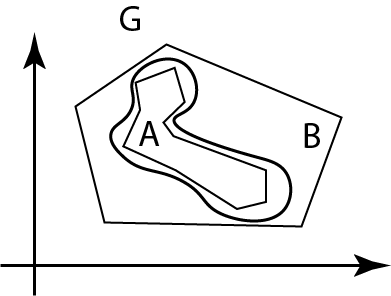
\includegraphics[scale=0.3]{graph17.png}\label{figure17}
        \end{center}
    \end{figure}
\end{definition}

\section{Измеримое по Жордану (квадрируемое) множество. Площадь.}

\begin{definition}
    Множество $G\subset\mathbb{R}^2$ называется \textbf{измеримым по Жардану} (или \textbf{квадрируемым}),
    если:
    \begin{equation*}
        S_* = \underset{A\subset G}{\sup} S(A) = S^* = \underset{B\supset G}{\inf}S(B),
    \end{equation*}
    где $\sup$ берется по всем многоугольникам, вписанным в $G$, а $\inf$ - по всем многоугольникам,
    описанным около $G$. При этом их общее значение $S = S_* = S^*$ называется \textbf{площадью} $G$,
    или \textbf{мерой Жардана}.
    \begin{center}
        $S_*$ - \textbf{внутренняя} мера, $S^*$ - \textbf{внешняя} мера.
    \end{center}

    Другими словами, множество $G\subset\mathbb{R}^2$ квадрируемо, если внутреняя и внешняя меры совпадают.

    Здесь $S(A),\ S(B)$ - площади многоугольников $A$ и $B$. Многоугольник $A$ можно разбить на конечное число
    прямоугольников и прямоугольных треугольников:
    \begin{figure}[h]
        \begin{minipage}[h]{0.49\linewidth}
            \center{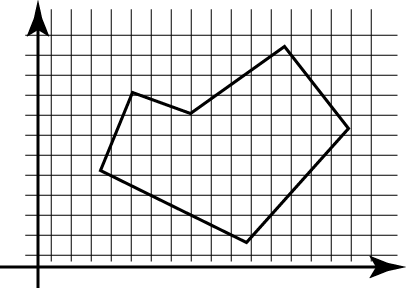
\includegraphics[scale=0.2]{graph18.png}}
        \end{minipage}
        \hfill
        \begin{minipage}[h]{0.49\linewidth}
            $S_\square = ab; \quad S_\triangle = \frac{1}{2}ab$
        \end{minipage}
    \end{figure}
\end{definition}

\begin{example}
    (из определения)

    \begin{enumerate}
        \item Квадрируемые множетсва на плоскости.

              Круг с границей:
              \begin{equation*}
                  x^2 + y^2 = 1
              \end{equation*}
              Упражнение: доказать, что круг - квадрируемое множество.
        \item Неквадрируемые множества на плоскости.

              Множество точек одинарного квадрата с рациональными координатами:
              \begin{equation*}
                  G = (\mathbb{Q} \times \mathbb{Q})\cap([0;1] \times [0;1])
              \end{equation*}
              Вписанный многоугольник $A = \emptyset, \ S(A) = 0$. Многоугольник $B = [0;1] \times [0;1]$
              имеет площадь равную  $1$ ($S(B) = 1$).
              \begin{equation*}
                  S_* = 0, \quad S^* = \underset{B'\supset G}{\inf}S(B') = S(B) = 1 \ (S_* \ne S^*)
              \end{equation*}
    \end{enumerate}
\end{example}

\section{Критерий квадрируемости множества}

\begin{theorem}[критерий квадрируемости]
    Множество $G\subset\mathbb{R}^2$ квадрируемо $\iff \forall \epsilon > 0 \ \exists$ многоугольники $A$ и $B$:
    \begin{enumerate}
        \item $A\subset G, \ B \supset G$,
        \item $S(B) - S(A) < \epsilon$.
    \end{enumerate}
\end{theorem}

\section{Криволинейная трапеция}

\begin{definition}
    \textbf{Криволинейная трапеция} - часть плоскости, ограниченная прямыми $x=a, \ x=b$, графиком функции
    $y = f(x)$ и осью $Ox$. {\Large РИСУНОК}
\end{definition}

\section{Квадрируемость криволинейной трапеции}

\begin{theorem}
    Криволинейная трапеция квадрируема и ее площадь равна:
    \begin{equation*}
        S = \int_{a}^{b}f(x)dx,
    \end{equation*}
    где $f(x)$ - непрерывна на $[a;b], \ f(x) \geqslant 0$.
\end{theorem}

\section{Квадрируемость криволинейного сектора}

\begin{definition}
    Фигура на плоскости, ограниченная лучами $\phi = \alpha$ и $\phi = \beta$ и кривой $\rho = \rho(\phi)$
    называется \textbf{криволинейным сектором}.
\end{definition}

\begin{theorem}
    Пусть криволинейный сектор $\Omega$ ограничен лучами $\phi = \alpha, \ \phi = \beta$ и кривой $\rho
        = \rho(\phi)$. Тогда:
    \begin{equation*}
        S(\Omega) = \frac{1}{2}\int_{\alpha}^{\beta}\rho^2(\phi)d\phi,
    \end{equation*}
    где $\rho(\phi)$ - непрерывна на $[\alpha;\beta]$. {\Large РИСУНОК}
\end{theorem}

\section{Несобственный интеграл, заданный на луче, на прямой, на отрезке.
  Сходящийся и расходящийся несобственный интеграл}

\begin{definition}
    Пусть $f:[a;+\infty)\rightarrow\mathbb{R}$ (задана на луче) и $\forall b \in [a;+\infty) \ f\in R[a;b]$.
    Рассмотрим:
    \begin{equation*}
        \underset{b\rightarrow+\infty}{\lim}\int_{a}^{b}f(x)dx,
    \end{equation*}
    этот предел называется \textbf{несобственным интегралом} от функции $f(x)$ на луче $[a;+\infty)$.

    Если этот предел существует и конечен, то несобственный интеграл называется \textbf{сходящимся}, иначе
    \textbf{расходящимся}. Обозначение:
    \begin{equation*}
        \int_{a}^{+\infty}f(x)dx \overset{def}{=}\underset{b\rightarrow+\infty}{\lim}\int_{a}^{b}f(x)dx
    \end{equation*}
\end{definition}

\begin{definition}
    (продолжение определения)

    \begin{enumerate}
        \item $\int_{2}^{+\infty}\frac{dx}{x^2} = \underset{b\rightarrow\infty}{\lim}\int_{2}^{b}\frac{dx}{x^2} =
                  \underset{b\rightarrow+\infty}{\lim}(F(b) - F(2)) = \underset{b\rightarrow+\infty}{\lim}(-\frac{1}{b} +
                  \frac{1}{2}) = \frac{1}{2}$.

              Аналогично, пусть функция $f:(-\infty;a]\rightarrow\mathbb{R}, \ f\in R[a;b], \ \forall b \in (-\infty;a]$.
              \begin{equation*}
                  \underset{b\rightarrow-\infty}{\lim}\int_{a}^{b}f(x)dx,
              \end{equation*}
              этот предел называется \textbf{несобственным интегралом} от функции $f(x)$ на луче $(\infty;a]$.

              Если этот предел существует и конечен, то соответственно несобственный интеграл - сходящийся. Обозначается:
              \begin{equation*}
                  \int_{-\infty}^{a}f(x)dx \overset{def}{=}\underset{b\rightarrow-\infty}{\lim}\int_{b}^{a}f(x)dx.
              \end{equation*}
              Аналогично:
              \begin{equation*}
                  \int_{-\infty}^{+\infty}f(x)dx = \int_{-\infty}^{a}f(x)dx + \int_{a}^{+\infty}f(x)dx = \underset{c
                      \rightarrow+\infty, b\rightarrow-\infty}{\lim}\int_{b}^{c}f(x)dx,
              \end{equation*}
              где $c\rightarrow+\infty, b\rightarrow-\infty$ - независимые друг от друга ($\forall b,c \ f(x)\in
                  R[b;c]$). {\Large РИСУНОК}

        \item Далее, пусть $f:[a;b)\rightarrow\mathbb{R}: \ \forall c \in [a;b) f\in R[a;c]$. Положим:
                          \begin{equation*}
                              \int_{a}^{b}f(x)dx = \underset{c\rightarrow b}{\lim}\int_{a}^{c}f(x)dx.
                          \end{equation*}
                          Эта величина называется \textbf{несобственным интегралом} от функции $f$ на полуинтервале $[a;b)$.

                                  Если предел существует, то несобственный интеграл называется \textbf{сходящимся}, иначе \textbf{расходящимся}.

                                  Аналогично, пусть $f:(a;b]\rightarrow\mathbb{R}$, причем $\forall c \in (a;b] \ f\in R[c;b]$:
              \begin{equation*}
                  \int_{a}^{b}f(x)dx \overset{def}{=} \underset{c\rightarrow a}{\lim}\int_{c}^{b}f(x)dx \ -
              \end{equation*}
              несобственный интеграл от функции $f(x)$ на полуинтервале $(a;b]$.

              Аналогично, пусть $f:(a;b)\rightarrow\mathbb{R}$, причем $\forall c,d \in (a;b) \ f\in R[c,d]$.
              Тогда:
              \begin{equation*}
                  \int_{a}^{b}f(x)dx \overset{def}{=} \underset{c\rightarrow a,d\rightarrow b}{\lim}\int_{c}^{d}
                  f(x)dx,
              \end{equation*}
              (где $c\rightarrow a,d\rightarrow b$ - независимые друг от друга) - несобственный интеграл от $f(x)$
              на $(a;b)$

        \item Пусть $f:[a;b]\rightarrow\mathbb{R}$ и $\exists c \in (a;b): \ f$ - неограниченана в точке $c$.
              \begin{equation*}
                  \int_{a}^{b} f(x) dx = \int_{a}^{c - \epsilon} f(x)dx + \int_{c+\epsilon}^{b}f(x)dx =
              \end{equation*}
              \begin{equation*}
                  \underset{\epsilon\rightarrow0}{\lim}\int_{a}^{c - \epsilon} f(x)dx + \underset{\epsilon}{\lim}
                  \int_{c+\epsilon}^{b}f(x)dx.
              \end{equation*}
              Если $\lim$ существует, то интеграл ялвяется сходящимся.

              В дальнейшем будем рассматривать:
              \begin{equation*}
                  \int_{a}^{\omega}f(x)dx,
              \end{equation*}
              где $\omega = +\infty, \ -\infty, \ b$.
    \end{enumerate}
\end{definition}

\section{Критерий Коши сходимости несобственного интеграла}

\begin{theorem}[Критерий Коши]
    Пусть $\forall b \in [a;\omega) \ f\in R[a;b]$.

    $\int_{a}^{\omega}f(x)dx$ сходится $\iff \ \forall
        \epsilon > 0 \ \exists B\in [a;\omega): \ \forall b_1,b_2 \in (a;\omega)$ и $b_1,b_2 > B$ верно неравенство:
    \begin{equation*}
        | \int_{b_1}^{b_2}f(x)dx | < \epsilon
    \end{equation*}
    {\Large РИСУНОК}
\end{theorem}

\section{Свойства несобственного интеграла}

\begin{theorem}
    Пусть $\forall b\in [a;\omega) \ f\in R[a;b]$.
    \begin{enumerate}
        \item Тогда $\int_{a}^{\omega}f(x)dx$ сходится $\iff \ \forall
                  b\in[a;\omega) \ \int_{b}^{\omega}f(x)dx$ сходится и
              \begin{equation*}
                  \int_{a}^{\omega}f(x)dx = \int_{a}^{b}f(x)dx + \int_{b}^{\omega} f(x)dx
              \end{equation*}
              {\Large РИСУНОК}
        \item
              \begin{equation*}
                  \underset{b\rightarrow\omega}{\lim}\int_{b}^{\omega}f(x)dx = 0
              \end{equation*}
        \item $\forall c \in \mathbb{R}$
              \begin{equation*}
                  \int_{a}^{\omega}cf(x)dx = c\int_{a}^{\omega}f(x)dx
              \end{equation*}
              (то есть если $c\int_{a}^{\omega}f(x)dx$ сходится, то сходится $\int_{a}^{\omega}c(x)dx$ и наоборот,
              и они равны)
        \item Если $\int_{a}^{\omega}f(x)dx$ и $\int_{a}^{\omega}g(x)dx$ сходятся, то сходится и
              \begin{equation*}
                  \int_{a}^{\omega}(f(x) + g(x))dx = \int_{a}^{\omega}f(x)dx + \int_{a}^{\omega}g(x)dx
              \end{equation*}
    \end{enumerate}
\end{theorem}

\section{Сходимость несобственного интеграла от неотрицательных функций}

\begin{theorem}[несобственная сходимость интеграла от неотрицательной функции]
    Пусть $f\in R[a;b]$ для $\forall b \in (a;\omega)$ и $f(x)\leqslant 0 \ \forall x \in [a;\omega).$

    $\int_{a}^{\omega}f(x)dx$ сходится $\iff \exists M > 0: \ \forall b \in (a;\omega)$
    \begin{equation*}
        \int_{a}^{b}f(x)dx < M.
    \end{equation*}
    {\Large РИСУНОК}
\end{theorem}

\section{Первый признак сравнения}

\begin{theorem}[первый признак сравнения]
    Если $\forall x \in [a;\omega) \ f(x) \leqslant g(x)$ и $\forall b \in [a;\omega) \ f,g \in R[a;b], \
        f(x) \geqslant 0, \ g(x) \geqslant 0$, тогда:
    \begin{enumerate}
        \item Если $\int_{a}^{\omega}g(x)dx$ - сходится $\implies \int_{a}^{\omega}f(x)dx$ - сходится.
        \item Если $\int_{a}^{\omega}f(x)dx$ - расходится $\implies \int_{a}^{\omega}g(x)dx$ - расходится.
    \end{enumerate}
\end{theorem}

\section{Второй признак сравнения}

\begin{theorem}[второй признак сравнения]
    Если $\forall x \in [a;\omega) \ f(x) > 0, \ g(x) > 0$ и $\exists \underset{x\rightarrow \omega}{\lim}
        \frac{f(x)}{g(x)} = A$ (либо $0$, либо $+\infty$, либо $const \ne 0$), тогда:
    \begin{enumerate}
        \item Если $A = +\infty$, то из расходимости $\int_{a}^{\omega}g(x)dx$ следует расходимость $\int_{a}^{\omega}
                  f(x)dx$, а из сходимости $\int_{a}^{\omega}f(x)dx$ следует сходимость $\int_{a}^{\omega}g(x)dx$.
        \item Если $A = 0$, то из расходимости $\int_{a}^{\omega}f(x)dx$ следует расходимость $\int_{a}^{\omega}
                  g(x)dx$, а из сходимости $\int_{a}^{\omega}g(x)dx$ следует сходимость $\int_{a}^{\omega}f(x)dx$.
        \item Если $A = const \ne 0$, то интегралы $\int_{a}^{\omega}f(x)dx$ и $\int_{a}^{\omega}g(x)dx$ ведут
              себя одинаково.
    \end{enumerate}
\end{theorem}

\section{Абсолютно сходящийся несобственный интеграл}

\begin{definition}
    Пусть $\forall b \in [a;\omega) \ f\in R[a;b]$.

    $\int_{a}^{\omega}f(x)dx$ называется \textbf{абсолютно сходящимся}, если сходится $\int_{a}^{\omega}|f(x)|dx$.
\end{definition}

\section{Связь сходимости и абсолютной сходимости несобственного интеграла}

\begin{theorem}
    Если $\int_{a}^{\omega}| f(x) |dx$ сходится, то $\int_{a}^{\omega}f(x)dx$ тоже сходится (или если интеграл
    абсолютно сходящийся, то он сходящийся).

    При этом:
    \begin{equation*}
        | \int_{a}^{\omega}f(x)dx | \leqslant \int_{a}^{\omega}| f(x) |dx
    \end{equation*}
\end{theorem}

\section{Признак Вейерштрасса}

\begin{effect}[признак Вейерштрасса]
    Если $\forall x \in [a;\omega) \ | f(x) | \leqslant g(x)$ и $\int_{a}^{\omega}g(x)dx$ сходится, то
    $\int_{a}^{\omega}f(x)dx$ сходится.
\end{effect}

\section{Условно сходящийся несобственный интеграл}

\begin{definition}
    Если $\int_{a}^{\omega}| f(x) |dx$ расходится, а $\int_{a}^{\omega}f(x)dx$ сходится, то $\int_{a}^{\omega}$
    называется \textbf{условно сходящимся}.
\end{definition}

\section{Признак Абеля}

\begin{theorem}[признак Абеля]
    Если:
    \begin{enumerate}
        \item $\int_{a}^{\omega}$ сходится,
        \item $g(x)$ монотонна и ограничена на $[a;\omega)$,
    \end{enumerate}
    то $\int_{a}^{\omega} f(x)g(x)dx$ - сходится.
\end{theorem}

\section{Признак Дирихле}

\begin{theorem}[признак Дирихле]
    Если:
    \begin{enumerate}
        \item Функция $F(b) = \int_{a}^{b}f(x)dx$ ограничена на $[a;\omega)$, то есть $\exists M > 0: \
                  \forall b \in[a;\omega)$
              \begin{equation*}
                  | \int_{a}^{b}f(x)dx | \leqslant M,
              \end{equation*}
        \item $g(x)$ - монотонна на $[a;\omega)$ и $g(x)\rightarrow 0$ при $x\rightarrow\omega$.
              Тогда $\int_{a}^{\omega}f(x)g(x)dx$ - сходится.
    \end{enumerate}
\end{theorem}

\section{Теорема о замене переменной в несобственном интеграле}

\begin{theorem}[о замене переменной в несобственном интеграле]
    Пусть $\forall b \in [a;\omega), \ f \in C[a;b]$ (множество непрерывных функций), функция $x = \phi(t):$
    \begin{enumerate}
        \item $\phi: \ [\alpha;\omega_1) \rightarrow [a;\omega)$,
        \item $\phi(\alpha) = a$, при $t \rightarrow \omega_1, \ \phi(t) \rightarrow \omega$,
        \item $\phi(t)$ монотонно возрастает на $[\alpha;\omega_1)$,
        \item $\phi'(t)$ непрерывна на $[\alpha;\omega_1)$,
    \end{enumerate}
    Тогда интегралы $\int_{a}^{\omega}f(x)dx$ и $\int_{\alpha}^{\omega_1}f(\phi(t))\phi'(t)dt$ ведут себя
    одинаково и равны между собой.
\end{theorem}

\section{Линейное пространство}

\begin{definition}
    \textbf{Линейным пространством} называется четверка $(X,K,+,*)$, где $X$ - множество, $K$ - поле, $"+"$ -
    операция сложения на $X$ ($"+": \ X \times X \rightarrow X$), $"*"$ - операция умножения элемента поля $K$
    на элемент множества $X$ ($"*": \ K \times X \rightarrow X$).

    При этом выполняются следующие аксиомы:
    \begin{enumerate}
        \item $<X,+>$ - абелева группа;
        \item
              \begin{enumerate}
                  \item $\forall \alpha,\beta \in K$ и $\forall x \in X \quad (\alpha\beta)x = \alpha(\beta X)$,
                  \item $\forall x,y \in X, \ \forall \alpha \in K \quad \alpha (x+y) = \alpha x + \alpha y$,
                  \item $\forall \alpha,\beta \in K, \forall x \in X \quad (\alpha + \beta)x = \alpha x + \beta x$,
                  \item $\forall x \in X, \ 1 \in K \quad 1x = x$.
              \end{enumerate}
    \end{enumerate}
\end{definition}

\section{Линейное нормированное пространство. Норма}

\begin{definition}
    \textbf{Линейным нормированным пространством} называется пара $(X,||*||)$, где $X$ - линейное пространство
    над полем $\mathbb{R}$, а $||*||$ - функция из $X$ в $\mathbb{R}$.

    $||*||: \ X \rightarrow \mathbb{R}$, причем выполнены следующие аксиомы для нее:
    \begin{enumerate}
        \item $||x|| = 0 \iff x = \overline{0}$ (читается "норма от $x$"),
        \item $\forall \lambda \in \mathbb{R} \ ||\lambda x|| = |\lambda| * ||x||$,
        \item $\forall x,y \in X \ ||x+y|| \leqslant ||x|| + ||y||$ (неравенство треугольника).
    \end{enumerate}
    Функция $||*||$ называется \textbf{нормой}.
\end{definition}

\section{Примеры линейных нормированных пространств (ЛНП)}

\begin{example}
    ЛНП:

    \begin{enumerate}
        \item $X = \mathbb{R}, \ \forall x \in X \quad ||x|| = |x|$ (норма = модулю по свойствам нормы),
        \item $X = \mathbb{R}^n = \mathbb{R} \times \mathbb{R} \times \ldots \times \mathbb{R}$ ($n$ раз),
              $\forall x \in X \ ||x|| = (\sum_{k=1}^{n}a_k^2)^\frac{1}{2}, \ x = (a_1,\ldots,a_n) \in X$.
              Покажем, что это норма:

              $1.,2.$ - очевидно. Докажем, что $\forall x,y \in X \ ||x+y|| \leqslant ||x||x + ||y||$, то есть
              докажем, что $(\sum_{k=1}^{n}(x_k + y_k)^2)^\frac{1}{2} \leqslant (\sum_{k=1}^{n}x_k^2)^\frac{1}{2}
                  + (\sum_{k=1}^{n}y_k^2)^\frac{1}{2} \ (\triangle)$.

              Рассмотрим $\sum_{k=1}^{n}(x_k + y_k)^2 = \sum_{k=1}^{n}x_k^2 + 2\sum_{k=1}^{n}x_k y_k + \sum_{k=1}^{n}
                  y_k^2 \leqslant |$ используем неравенство Назарова-Заблоцкого (Коши-Буньковского) $ \sum_{k=1}^{n}x_k y_k \leqslant
                  (\sum_{k=1}^{n}x_K^2)^\frac{1}{2}(\sum_{k=1}^{n}y_k^2)^\frac{1}{2}| \leqslant \sum_{k=1}^{n}x_k^2 +
                  2(\sum_{k=1}^{n}x_k^2)^\frac{1}{2}(\sum_{k=1}^{n}y_k^2)^\frac{1}{2} + \sum_{k=1}^{n}y_k^2 =
                  [(\sum_{k=1}^{n}x_k^2)^\frac{1}{2} + (\sum_{k=1}^{n}y_k^2)^\frac{1}{2}]^2$.

              Имеем:
              \begin{equation*}
                  \sum_{k=1}^{n}(x_k + y_k)^2 \leqslant [(\sum_{k=1}^{n}x_k^2)^\frac{1}{2} + (\sum_{k=1}^{n}y_k^2)^\frac{1}{2}]^2 \implies
              \end{equation*}
              приходим к $(\triangle)$ операцией взятия корня от обеих частей неравенства
              \begin{equation*}
                  \implies (\sum_{k=1}^{n}(x_k + y_k)^2)^\frac{1}{2} \leqslant (\sum_{k=1}^{n}x_k^2)^\frac{1}{2} +
                  (\sum_{k=1}^{n}y_k^2)^\frac{1}{2}.
              \end{equation*}
        \item $X = \mathbb{R}^n, \ \forall x = (x_1,\ldots,x_n)\in X \quad ||x|| = \underset{k=\overline{1,n}}{\max}
                  |x_k|$.

              \begin{center}
                  Такое ЛНП обозначается $\mathbb{R^n_\infty}$.
              \end{center}
        \item $X = \mathbb{R}^n, \ \forall x = (x_1,\ldots, x_n) \in X \quad ||x|| = (\sum_{k=1}^{n}x_k^p)^\frac{1}{p},
                  \ p > 1$.

              Упражнение: доказать, что введенная функция есть норма, используя неравенство Левановича (Гельдера):
              \begin{equation*}
                  \sum_{k=1}^{n}x_k y_k \leqslant (\sum_{k=1}^{n}x_k^p)^\frac{1}{p} (\sum_{k=1}^{n}y_k^p)^\frac{1}{p}.
              \end{equation*}

        \item $X$ - пространство непрерывных на $[a;b]$ функций, то есть $X = C[a;b], \ \forall x \in X
                  \quad ||x|| = \underset{t \in [a;b]}{\max}|x(t)|$; 1,2,3 - почти очевидно.

        \item $X = C[a;b], \ \forall x \in X \quad ||x|| = \int_{a}^{b}|x(t)|dt$.

              Покажем, что введенная функция есть норма:
              \begin{enumerate}
                  \item $||x(t)|| = 0 \iff x(t) = 0$;

                        Пусть $\int_{a}^{b}|x(t)|dt = 0$. От противного. Допустим, что $\exists t_0 \in [a;b]: \ x(t_0) \ne 0$.
                        Тогда $\exists t_0 \in [\alpha;\beta], \ [\alpha;\beta] \subset [a;b]$ и $\forall t \in [\alpha;\beta]
                            \quad |x(t)| > 0$,
                        \begin{equation*}
                            \int_{a}^{b}x(t)|dt \geqslant \int_{\alpha}^{\beta}|x(t)|dt
                        \end{equation*}
                        Противоречие $\implies \forall t \in [a;b] \ |x(t)| = 0$.

                  \item $|| \lambda x || = | \lambda | * || x ||$ (из свойств определенного интеграла);
                  \item $|| x+y || \leqslant || x || + || y ||$ (из свойств определенного интеграла);
              \end{enumerate}
        \item $X = C[a;b]$.
    \end{enumerate}
\end{example}

\section{Метрика ЛНП}

ЛНП ($C[a;b], || x || (*)$) образначается $C^p[a;b]$.

\begin{statement}
    Пусть $(X,|| * ||)$ - ЛНП. Тогда функция $\rho X \times X \rightarrow \mathbb{R}$, опредленная $\rho(x,y)
        = || x-y ||$, является метрикой ЛНП.
\end{statement}

\section{Банахово ЛНП. Примеры}

\begin{definition}
    Если линейное нормированное пространство является полным относительно введенной метрики, то оно называется
    \textbf{банахово}.

    ($X$ - полное, если $\forall$ фундаментальная последовательность сходится).
\end{definition}

\begin{example}
    (банаховых пространств)

    \begin{enumerate}
        \item $X = \mathbb{R}$ - банахово;
        \item $X = C[a;b], \ ||x|| = \underset{t \in [a;b]}{\max}|x(t)|$;
        \item $C_p[a;b]$ - ЛНП, $X = C[a;b]$,
              \begin{equation*}
                  ||x|| = (\int_{a}^{b}|x(t)|^p dt)^\frac{1}{p}.
              \end{equation*}
    \end{enumerate}
\end{example}

\section{Теорема о вложенных шарах}

\begin{theorem}[о вложенных шарах]
    Метрическое пространство (МП) является полным $\iff \forall$ последовательность вложенных замкнутых шаров,
    радиусы которых стремятся к нулю, имеют в нем непустое пересечение.
\end{theorem}

\section{Сжимающее отображение}

\begin{definition}
    Пусть $(X,\rho_X), \ (Y,\rho_Y)$ - МП. Отображение $f:X\rightarrow Y$ называется \textbf{сжимающим},
    если $\exists 0 \leqslant \alpha < 1: \ \forall x_1,x_2 \in X$
    \begin{equation*}
        \rho_Y(f(x_1),f(x_2)) \leqslant \alpha * \rho_X(x_1,x_2).
    \end{equation*}
\end{definition}

\section{Принцип сжимающих отображений}

\begin{theorem}[принцип сжимающих отображений]
    Сжимающее отображение полного МП в себя имеет единственную неподвижную точку, то есть если
    $(X,\rho)$ - полное, отображение $f:X\rightarrow X$ - сжимающее, то
    \begin{equation*}
        \exists ! a \in X: \quad f(a) = a.
    \end{equation*}
\end{theorem}

\section{Предкомпактное множество в МП}

\begin{definition}
    Множество $E$ в метрическом пространстве называется \textbf{предкомпактным} (\textbf{относительно компактным}),
    если ее замыкание $\overline{E}$ компактно.
\end{definition}

\section{Вполне ограниченное множество}

\begin{definition}
    Множество $E$ в МП $(X,\rho)$ называется \textbf{вполне ограниченным}, если $\forall \epsilon > 0 \ \exists$
    конечная $\epsilon$-сеть для $E$.

    Напоминание: $\epsilon$-сеть - набор $\{x_1,\ldots,x_n \ | \ x_i \in E\} \ \forall x \in E \ \exists$ хотя бы
    одна точка $x_i: \ \rho(x,x_i) < \epsilon$.
\end{definition}

\section{Теорема Хаусдорфа}

\begin{theorem}[Хаусдорфа]
    Множество $E$ в полном МП $(X,\rho)$ ялвяется предкомпактным $\iff$ оно вполне ограничено.
\end{theorem}

\section{Теорема о полноте $\mathbb{R}^n$}

\begin{theorem}
    Пространство $\mathbb{R}^n$ (n-мерное линейное пространство с евклидовой метрикой),
    \begin{center}
        $||x|| = (\sum_{i=1}^{n} (x^i)^2)^\frac{1}{2}$ - полное
    \end{center}
\end{theorem}

\section{Критерий компактности $\mathbb{R}^n$}

\begin{theorem}[критерий компактности в $\mathbb{R}^n$]
    Множество $E \subset \mathbb{R}^n$ компактно $\iff$ замкнуто и ограничено.
\end{theorem}

\section{Эквивалентность норм в $\mathbb{R}^n$}

\begin{definition}
    Пусть $(X, ||*||_1),(X, ||*||_2)$ - линейное нормированное пространство (конечномерное). Говорят, что $||*||_1
        \sim ||*||_2$ (эквивалентны), если $\exists c_1,c_2 > 0 \ (c_1,c_2 \in \mathbb{R}):$
    \begin{equation*}
        \forall x \in X \quad c_1 * ||x||_2 \leqslant ||x||_1 \leqslant c_2 * ||x||_2 \quad (*)
    \end{equation*}
\end{definition}

\begin{theorem}[эквивалентность норм в конечномерном пространстве]
    Если $X$ - конечномерное пространство МП, и $||*||_1, \ ||*||_2$ - две нормы на нем, то:
    \begin{equation*}
        ||*||_1 \sim ||*||_2
    \end{equation*}
\end{theorem}

\section{Линейные отображения в конечномерных пространствах}

\begin{definition}
    Пусть $X,Y$ - линейные пространства. Отображение $L: X \rightarrow Y$ называется \textbf{линейным}, если
    $\forall x_1,x_2 \in X$ и $\alpha,\beta \in \mathbb{R}$:
    \begin{equation*}
        L(\alpha x_1 + \beta x_2) = \alpha * L(x_1) + \beta L(x_2) = \alpha L x_1 + \beta L x_2.
    \end{equation*}
\end{definition}

\section{Теорема о матрице линейного отображения}

\begin{theorem}
    Всякому линейному отображению $L:\mathbb{R}^n \rightarrow \mathbb{R}^k$ можно поставить в соответствие
    матрицу $A$ размером $k \times n$:
    \begin{equation*}
        \forall x \in \mathbb{R}^n \quad L(x) = Ax.
    \end{equation*}

    При этом, если в $\mathbb{R}^n$ и $\mathbb{R}^k$ зафиксированны базисы, то матрица $A$ определяется однозначно.
\end{theorem}

\section{Теорема о непрерывности линейного отображения}

\begin{statement}
    Если $L:\mathbb{R}^n \rightarrow \mathbb{R}^k$ - линейно, то оно непрерывно.
\end{statement}

\section{Дифференциал в точке в $\mathbb{R}^n$}

\begin{definition}
    Пусть $D \subset \mathbb{R}^n, \ f:D\rightarrow\mathbb{R}^k$, точка $a\in D$ - предельная точка для $D$.

    Отображение $f$ называется \textbf{дифференцируемым} в точке $a$, если $\forall h: \ a+h \in D \ \exists$
    линейное отображение $L(a):\mathbb{R}^n\rightarrow\mathbb{R}^k:$
    \begin{equation*}
        f(a+h) - f(a) = L(a)h + o(h), \quad h\rightarrow\overline{0}.
    \end{equation*}

    Линейный оператор $L(a)$ называется \textbf{дифференциалом} (или \textbf{касательным отображением}, или
    \textbf{производным отображением}) функции $f$ и обозначается:
    \begin{equation*}
        Df(x), \quad df(x)
    \end{equation*}
\end{definition}

\section{Критерий дифференцируемости отображения в $\mathbb{R}^n$}

\begin{statement}
    Пусть $f:D\rightarrow\mathbb{R}^k, \ D \subset \mathbb{R}^n, \ a \in D$ \\ и $f(x) = \left(
        \begin{array}{c}
                f^1(x) \\
                f^2(x) \\
                \vdots \\
                f^k(x)
            \end{array}
        \right) = \left(
        \begin{array}{c}
                f^1(x^1,x^2,\ldots,x^n) \\
                f^2(x^1,x^2,\ldots,x^n) \\
                \vdots                  \\
                f^k(x^1,x^2,\ldots,x^n) \\
            \end{array}
        \right)$

    Отображение $f$ дифференцируемо в точке $a \iff$ отображение $f^i: D \rightarrow \mathbb{R}$ дифференцируемо
    в точке $a$.
\end{statement}

\section{Область}

\begin{definition}
    Множество $D\subset\mathbb{R}^n$ называется \textbf{областью}, если оно открыто и линейно связно.
\end{definition}

\section{Частная производная функции многих переменных}

\begin{definition}
    Пусть $D$ - область в $\mathbb{R}^n, \ f:D\rightarrow\mathbb{R},$
    \begin{equation*}
        f(x) = f(x^1,x^2,\ldots,x^n), \quad x \in D.
    \end{equation*}

    \textbf{Частной производной} отображения $f$ точки $x \in D$ по переменной $x^i$ называется
    \begin{equation*}
        \underset{h^i\rightarrow 0}{\lim}\frac{f(x^1,x^2,\ldots,x^i + h^i, \ldots,x^n) - (f(x^1,x^2,\ldots,x^n))}{h^i},
    \end{equation*}
    если этот предел существует.

    Обозначение:
    \begin{equation*}
        \frac{\partial f}{\partial x^i} \quad or \quad f_{x^i}'
    \end{equation*}
\end{definition}

\section{Связь дифференциала и частных производных}

\begin{theorem}[о связи дифференциала и частных производных]
    Если $f:D\rightarrow\mathbb{R}$ ($D$ - область в $\mathbb{R}^n$) дифференцируема в точке $x \in D$, то она
    имеет в точке $x$ все частные производные, при этом:
    \begin{equation*}
        df(x)h = \frac{\partial f}{\partial x^1}h^1 + \frac{\partial f}{\partial x^2}h^2 + \ldots +
        \frac{\partial f}{\partial x^n}h^n =
    \end{equation*}
    \begin{equation*}
        =\left(\begin{array}{cccc}
            \frac{\partial f}{\partial x^1} & \frac{\partial f}{\partial x^2} & \ldots & \frac{\partial f}{\partial x^n}
        \end{array}\right) * \left(\begin{array}{c}
            h^1    \\
            h^2    \\
            \vdots \\
            h^n
        \end{array}\right)
    \end{equation*}

    (здесь везде $1,2,\ldots,n$ - индексы, а не степени или производные).
\end{theorem}

\section{Матрица Якоби}

Пусть $f:\mathbb{R}^n \rightarrow \mathbb{R}^k$.

\textbf{Матрицей Якоби} отображения $f$ в точке $x\in\mathbb{R}$ называется:
\begin{equation*}
    \mathfrak{I}(x) = \left(
    \begin{array}{ccc}
            \frac{\partial f^1}{\partial x^1} & \ldots & \frac{\partial f^1}{\partial x^n} \\
            \frac{\partial f^2}{\partial x^1} & \ldots & \frac{\partial f^2}{\partial x^n} \\
            \vdots                            & \ddots & \vdots                            \\
            \frac{\partial f^k}{\partial x^1} & \ldots & \frac{\partial f^k}{\partial x^n}
        \end{array}
    \right)
\end{equation*}

Здесь $f(x) = \left(
    \begin{array}{c}
            f^1(x) \\
            \vdots \\
            f^k(x)
        \end{array}
    \right)$

Т. обр. $df(x)h = \mathfrak{I}(x)h = \left(
    \begin{array}{ccc}
            \frac{\partial f^1}{\partial x^1} & \ldots & \frac{\partial f^1}{\partial x^n} \\
            \frac{\partial f^2}{\partial x^1} & \ldots & \frac{\partial f^2}{\partial x^n} \\
            \vdots                            & \ddots & \vdots                            \\
            \frac{\partial f^k}{\partial x^1} & \ldots & \frac{\partial f^k}{\partial x^n}
        \end{array}
    \right) * \left(
    \begin{array}{c}
            h^1    \\
            \vdots \\
            h^k
        \end{array}
    \right) = \left(
    \begin{array}{ccc}
            df^1(x)h \\
            df^2(x)h \\
            \vdots   \\
            df^k(x)h
        \end{array}
    \right)$

Часто матрицу Якоби отображения $f$ будем обозначать $f'$.

\section{Дифференцируемость и арифметические операции}

\begin{theorem}
    Пусть $D\subset \mathbb{R}^n$ - область, $f:D\rightarrow\mathbb{R}^k, \ g:D\rightarrow\mathbb{R}^k,$ если
    $f$ и $g$ дифференцируемы в точке $x\in D$, то $\forall \lambda_1,\lambda_2\in\mathbb{R}$ функция
    $\lambda_1 f + \lambda_2 g$ дифференцируема в точке $x$, при этом:
    \begin{equation*}
        (\lambda_1f + \lambda_2g)' = \lambda_1f' + \lambda_2g',
    \end{equation*}
    где $(\lambda_1f + \lambda_2g)', \ f', \ g'$ - матрицы Якоби.
\end{theorem}

\section{Дифференцирование композиции}

\begin{theorem}[дифференцирование композиции]
    Пусть $X$ - область в $\mathbb{R}^n$, $Y$ - область в $\mathbb{R}^m, \ f:X\rightarrow Y, \ g:Y\rightarrow\mathbb{R}^k$.

    Если $f$ дифференцируема в точке $x \in X, \ g$ - дифференцируема в точке $y = f(x) \in Y$, то $g \circ f$ дифференцируема в точке $x$ и $(g \circ f)'(x) = g'(y) \cdot f'(x)$.
\end{theorem}

\section{Дифференцирование обратного отображения}

\begin{theorem}[о дифференцируемости обратного отображения]
    Пусть $D$ - область в $\mathbb{R}^n, \ f: D \rightarrow \mathbb{R}^n:$
    \begin{enumerate}
        \item $f$ дифференцируемо в точке $x \in D$;
        \item $f$ имеет обратное отображение в $D$;
        \item $f^{-1}$ - непрерывно в точке $y = f(x)$;
        \item $f'(x)$ - обратимая матрица.
    \end{enumerate}

    Тогда $f^{-1}:f(D)\rightarrow D$ дифференцируемо в точке $y = f(x)$ и $(f^{-1})' = [f'(x)]^{-1}$.
\end{theorem}

\end{document}